\section{Introduction} % ================== 

Tobler's First Law of Geography says that things close together in space tend to behave more similarly than things further apart \citep{Tobler1970}. The model fit in Chapter 3 fits well, at least according to the Hosmer-Lemeshow test, but there remains unexplained spatial variation in the mean. To account for the unexplained variation (possibly due to missing covariates), we augment the model with a spatially correlated random effect, giving a Spatial Generalized Linear Mixed Model (SGLMM) \citep{Banerjee2008}.

Broadly speaking, we add a spatial random effect to improve the model by attempting to model residual spatial correlation. More narrowly, as a first step in that process, the research in this chapter examines three procedures and their effectiveness for fitting big data SGLMMs on a personal computer (PC).

This chapter consists of four sections. The first section covers three topics for the remaining sections:  SGLMMs and Gaussian Random Fields (GRFs), big spatial data computational burdens, and Markov Chain Monte Carlo. The remaining three sections detail three approaches to dealing with the computational burdens of fitting our SGLMM: computational optimization, dimension reduction, and approximation.

\subsection{Spatial Generalized Linear Mixed Model (SGLMM)} % ======= ==========

In this chapter we fit models to hitter Jhonny Peralta only, and therefore drop hitter index $j$ (although we expect model parameters to depend on $j$). 

Let $\pmb{w}(\pmb{s}) = (w(\pmb{s}_{1}), w(\pmb{s}_{2}), \dots, w(\pmb{s}_{N}))$  be a vector of spatial random effects, where $w(\pmb{s}_{i})$ is the spatial random effect at location $\pmb{s}_{i}$. Adding the spatial random effect to the linear predictor in equation \ref{eq:glm} gives the following SGLMM:
\begin{equation} \label{eq:SGLMM}
Y_{i}|\mathbf{X}_{i}(\mathbf{s}_{i}) \stackrel{ind}{\sim} \mbox{Bernoulli}(\pi_{i}) 
\end{equation}
with
\begin{equation} \text{logit}(\pi_{i}|\pmb{s}_{i}) = \mathbf{X}_{i}(\mathbf{s}_{i})\beta + w(\pmb{s}_{i}),
\end{equation}
for swings $i = 1, 2, \dots, N$.

A Gaussian random field (GRF) provides a tractable structure for an $n \times 1$ vector of random effects such as $\pmb{w}(\pmb{s})$ \citep{Gelfand2010}. Accordingly, for vector of locations $\pmb{s} \in \pmb{D} \subseteq \pmb{R}^{2}$, with spatial domain $\pmb{D}$ (hitting zone): let $\pmb{w}(\pmb{s})$ be a multivariate Normal random vector, with mean $\pmb{0}$; and symmetric, positive definite covariance matrix $\Sigma(\pmb{\theta})$, with covariance parameters $\pmb{\theta}$ \citep{Haran2011}. That is,
\begin{equation} \label{eq:w}
\pmb{w}(\pmb{s}) | \pmb{\theta} \sim MVN(\pmb{0}, \Sigma(\pmb{\theta})). 
\end{equation}
In the following sections (\ref{stanopt} and \ref{ppm}) we use an isotropic spatial exponential covariance structure for $\Sigma(\pmb{\theta})$. In the exponential covariance model the ($i^{th},k^{th}$) element of the matrix $\pmb{\Sigma}(\pmb{\theta})$---the covariance of the random effects $w(\pmb{s}_{i})$ and $w(\pmb{s}_{k})$---is defined as:
\begin{equation} \label{eq:exp}
\Sigma(\phi, \sigma^{2})_{i,k} = \text{Cov}(w(\pmb{s}_{i}), w(\pmb{s}_{k})) =  \sigma^{2} \text{exp}(-||\pmb{s}_{i} - \pmb{s}_{k}||/\phi),
\end{equation}
with scale parameter $\sigma^{2}$, range parameter $\phi$, and where $||\pmb{s}_{i} - \pmb{s}_{k}||$ denotes the Euclidean distance between $\pmb{s}_{i}$ and $\pmb{s}_{k}$.

This spatial model, containing a latent (unobserved) Gaussian random field, gives $\pmb{Y}$, the swing outcome (Bernoulli) random variable, a complicated correlation structure. Bayesian hierarchical spatial models most effectively accommodate this structure, and Markov chain Monte Carlo (MCMC) methods most effectively estimate model parameters \citep{Banerjee2014}. High dimensionality for this spatial model induces substantial computational costs, referred to as the ``Big N problem'' \citep{Lindgren2011}.

\subsection{Three Approaches to the ``Big N Problem''}

Fitting the SGLMM in \ref{eq:SGLMM} involves evaluating the probability distribution function of $\pmb{w}$. In our case, the multivariate Normal probability distribution function for $\pmb{w}$ is:
\begin{equation} \label{eq:mvn}
f(\pmb{w}) = \frac{1}{(2\pi)^{n/2}|\Sigma|^{1/2}} \text{exp}\{ -\frac{1}{2}\pmb{w}'\Sigma^{-1}\pmb{w} \},
\end{equation}
where $|\Sigma|^{1/2}$ denotes the square root of the determinant of the n $\times$ n covariance matrix, and $\Sigma^{-1}$ denotes its inverse. For large sample sizes, these two components of the MVN distribution lead to prohibitive computational costs.

% For a sequence of two increasing functions $f(n)$ and $g(n)$, we say $f(n) = \mathcal{O}(g(n))$ as $n \rightarrow \infty$, if and only if there exists some $n_{0}$ and a positive real number M such that
%   $$|f(n)| \leq \text{M} \cdot |g(n)| \text{ for all } n \geq n_0. $$
% In words, $\mathcal{O}(g(n))$ is read ``big oh of g(n).'' 
The computational costs of fitting a SGLMM with a latent GRF increase at a rate of $\mathcal{O}(n^{3})$ \citep{Finley2009}. That is, for time  required to fit our model to $n$ observations, $t(n)$, there exists an $M > 0$ such that:
$$t(n) \leq M \cdot n^{3} \text{ as } n \rightarrow \infty.$$
In less technical terms, this means the upper bound on the amount of time required for model fitting increases at the same rate as $n^{3}$. To understand why, refer back to the MVN pdf in equation \ref{eq:mvn}, and notice the n $\times$ n covariance matrix inverse and the determinant. Every MCMC algorithm iteration requires calculation and construction of these components; this accounts for the $\mathcal{O}(n^{3})$ rate of increase, prohibitively slow model fitting, and the ``Big N'' problem. Recall our baseball data set contains $N = 9177$ Jhonny Peralta swings, and the full data set contained approximately 1.5 million swings.

To address these computational challenges, we used three model-fitting approaches.
\begin{enumerate}
\item Computational optimization in Bayesian computing software Stan \citep{rstan}.
\item Dimension reduction with Predictive process models, implemented in R with the R package {\bf spBayes} \citep{Eidsvik2012}, \citep{Finley2013}.
\item Integrated Nested Laplace Approximations \citep{Rue2009} with Stochastic Partial Differential Equations \citep{Lindgren2011}, implemented in the R with the package \verb|INLA-R| \citep{Lindgren2015}.
\end{enumerate}

\subsection{Markov Chain Monte Carlo (MCMC)}

MCMC methods are integral to applied Bayesian statistics. In Bayesian statistics we seek the posterior distribution of the parameter(s) of interest, given the observed data. The fundamental Bayesian proportionality, for observation vector $\pmb{y}$, and parameter vector $\theta$, takes the form \citep{Gelman2014}:
\begin{equation} \label{eq:bayes}
p(\pmb{\theta}|\pmb{y}) \propto f(\pmb{y}|\pmb{\theta})p(\pmb{\theta}).
\end{equation}
Elementary Bayesian models sometimes yield closed form posterior distributions, but more complex models rarely do. For complex models, MCMC offers an iterative procedure that, upon convergence, yields draws from the true posterior distribution. MCMC has its challenges and weaknesses, but, with sufficient computing power and time, often provides good estimates of the desired posterior distribution. 

Markov chain properties supply the critical theoretical components of MCMC. Foremost among them, a sequence of (possibly multivariate) random variables $\pmb{X}_{1}, \pmb{X}_{2}, \hdots \pmb{X}_{n}$ possesses the Markov property if the distribution of $\pmb{X}_{n+1}|\pmb{X}_{1}, \pmb{X}_{2}, \hdots , \pmb{X}_{n}$ depends only on $\pmb{X}_{n}$. A sequence of random variables with the Markov property constitutes a Markov chain. MCMC algorithms use Markov chains with additional, necessary properties that ensure that an equilibrium distribution exists \citep{Brooks2011}. If such an equilibrium distribution exists for a particular MCMC, then that equilibrium distribution is equivalent to the posterior distribution of interest.

The first two Bayesian estimation procedures in this chapter use a Metropolis sampling algorithm \citep{Metropolis1953}. The R package {\bf rstan} uses Hamiltonian Monte Carlo (HMC) sampling and a ``Metropolis reject step'' \citep{rstan}; while the R package {\bf spBayes} uses a ``Metropolis-within-Gibbs'' sampler \citep{Finley2013}. 

\section{Optimization in Stan} \label{stanopt} % =================

\subsection{Introduction}

Stan is a well known, ``state of the art platform'' for Bayesian statistical analysis and model fitting \citep{stanwebsite}, with an R interface \citep{rstan}. We hoped for sufficient speed based on its reputed efficient statistical and programming techniques, such as using a Hamiltonian Monte Carlo method and incorporating the lower level programming language C++. In the next few sections we describe HMC in detail to help understand why Stan is a good starting point, discuss techniques for fast implementation, and present results.

\subsection{Hamiltonian Monte Carlo (HMC)} 

Stan uses the Metropolis algorithm, which requires a proposal generating mechanism or a proposal distribution at each step. Often a random walk distribution, or some other accessible distribution, plays this role. On the other hand, Stan uses a proposal mechanism that originated in physics, HMC, to generate proposals for the Metropolis reject step. HMC generates well-mixed, high probability proposals---two important factors. Mixing refers to the degree to which proposals explore the parameter space, and acceptance rates refer to the likelihood that the algorithm accepts proposals. Insufficient mixing and low acceptance rates delay, or even prevent, the Markov chain from converging to its equilibrium distribution. On the other hand, an acceptance rate too high signals insufficient mixing and potentially overly correlated draws. In Stan's MCMC, HMC balances the proposal mechanism demands well \citep{Neal2011}. 

HMC history essentially unfolded in four stages. First, \cite{Metropolis1953} developed MCMC while conducting research into molecular states. Second, \cite{Alder1959} introduced {\it Hamiltonian dynamics} as an alternate representation of Newtonian mechanics, while modeling molecular motion as a deterministic process \citep{Newt}. Third, almost 30 years later, \cite{Duane1987} combined the two methods to create ``hybrid Monte Carlo,'' for simulating quantum mechanical processes. Over time, the name morphed into {\it Hamilton} Monte Carlo (HMC). Fourth, eventually HMC made its way into statistics, when \cite{Neal1996} used HMC to study neural networks.

To understand HMC, imagine a solid disk with known position and momentum on a frictionless surface, then randomly changing the momentum of the disk to alter its course, and calculating the new position. HMC treats the variables of interest as position variables, and uses randomly generated auxiliary Gaussian variables to change the momentum. Then, the new position, calculated with a set of differential equations, provides proposals for Metropolis updates. The differential equation solutions estimate trajectories of the hypothetical physical object (the disk), which then occupies a new position after a time step of some chosen duration. This crafty formulation provides distant (well mixed), yet high probability (high acceptance rate) proposals. This contrasts favorably with the random walk proposal generation process commonly used.\footnote{I dedicate this section to my high school physics teacher, the late William T. Meyers. He helped instill in me a love of physics, and emphasized that in his class we would learn critical thinking skills that we could use in our life.}

\subsection{The Hamilton Equations} % =================

This section uses the notation of \cite{Neal2011}. To define the Hamilton equations for d variables of interest, let d-dimensional position vector $q(t)$ depend on time $t$; and let $U(q(t))$ denote the potential energy at time $t$. Let $p(t)$ give the d-dimensional momentum at time $t$, and $K(p(t))$ denote kinetic energy at time $t$. Then the Hamilton equation,
\begin{equation}
H(q(t),p(t)) = U(q(t)) + K(p(t)),
\end{equation}
measures the total energy of a system as a function of potential and kinetic energy. 

In HMC applications, we let the potential energy, $U(q)$, be minus the log of the probability density function of interest, plus a constant.\footnote{We omit $t$ for clarity of presentation, here and elsewhere, but position and momentum remain functions of time $t$.} Next, define d-dimensional vector $p$ as a zero mean Gaussian random variable with covariance matrix M, and define $K(p)$ as minus the log of the multivariate Gaussian probability density function. This gives the Hamilton equation form:
\begin{equation} \label{eq:ham}
H(q,p) = -\text{log}f_{q}(q) + p^{T}\pmb{M}^{-1}p/2.
\end{equation}
This formulation yields tractable partial derivatives for calculating the change in position and momentum through time. For $i = 1,\dots, \text{d}$:
\begin{align}
\frac{d q_{i}(t)}{dt} &= \frac{\partial H}{\partial p_{i}}, \\
\frac{d p_{i}(t)}{dt} &= -\frac{\partial H}{\partial q_{i}}.
\end{align}
Substituting equation \ref{eq:ham} and simplifying gives:
\begin{align}
\frac{d q_{i}(t)}{dt} &=  [\pmb{M}^{-1}p]_{i} \\
\frac{d p_{i}(t)}{dt} &= \frac {\partial \left[ \text{log}f_{q}(q) \right]}{\partial q_{i}}
\end{align}
The differential equation solutions give the position and momentum at time t. With solutions in hand, the ``leapfrog method'' calculates changes in the Hamilton through small time steps, by discretizing the continuously defined Hamilton equation using Taylor Series approximations \citep{Neal2011}. 

In summary, the HMC algorithm samples from the auxiliary Normal distribution, and then calculates the proposal as the positions vector in the Hamilton equation. This method yields high probability, well mixed Metropolis proposals. This combination, and Stan's efficient Bayesian model fitting, motivated us to use Stan for model fitting.

\subsection{Optimization Techniques} % =================
With the techniques presented in this section, we aimed to improve Stan model fitting efficiency enough to successfully fit our SGLMM to thousands, or tens of thousands, of observations. The techniques include Bayesian, linear algebra, and purely computational strategies. We start with techniques related to the Bayesian model components.

Stan permits users to omit prior distributions for parameters, but then assumes a non-informative, uniform prior for that parameter. However, prominent Bayesian statistician and Stan developer Andrew Gelman pointed out in personal correspondence that the exponential covariance range parameter, $\phi$ in equation \ref{eq:exp}, requires an informative prior for model identifiability (uniqueness) \citep{Gelman2014}. In this vein, Stan developer Rob Trangucci recommended, also in personal correspondence, a sharp tailed prior distribution for range parameter $\phi$, such as the normal or log-normal, to act as soft upper and lower bound constraints \citep{Trangucci}. Even further, for practical computing time and convergence considerations, Trangucci indicated complex models---such as spatial hierarchical models---require proper priors for all $\beta$ coefficients \citep{Trangucci}. The next two techniques combine linear algebra and computational considerations.

For all operations in Stan, matrix algebra and vectors achieve greater speed and efficiency than loops and scalars \citep{STANtheMan}. For example, 
\begin{verbatim}
hit ~ bernoulli_logit(X*beta + Z)
\end{verbatim}
runs faster than
\begin{verbatim}
for (n in 1:N)
        hit[n] = bernoulli_logit(X[n]*beta[n] + Z[n])
\end{verbatim}
The first, faster line includes N$\times$1 column vectors \verb|hit|, \verb|beta|, and \verb|Z|; and N$\times$p matrix \verb|X|. The second, slower snippet, instead uses scalars \verb|hit[n]|, \verb|beta[n]|, and \verb|Z[n]|; and 1$\times$p row vector \verb|X[n]|.

Trangucci also suggested a QR factorization on covariate matrix $\pmb{X}$, in the linear predictor, to increase computational efficiency \citep{Trangucci}. A QR factorization consists of factoring an n $\times$ p matrix into the product of an n $\times$ p orthogonal matrix $\pmb{Q}$ and a p $\times$ p upper triangular matrix $\pmb{R}$, such that $\pmb{X} = \pmb{QR}$. Leveraging this factorization into a speed increase requires a reparameterization. To this end, let $\pmb{\theta} = \pmb{R \beta}$, which gives:
\begin{align}
\pmb{X} &= \pmb{QR} \\
\pmb{X \beta} &= \pmb{QR \beta} \\
\pmb{X \beta} &= \pmb{Q \theta},
\end{align}
and the model
\begin{equation} \label{eq:reparam}
\text{logit}(p_{i}|\pmb{s}_{i}) = \pmb{Q}_{i}(\pmb{s}_{i}) \pmb{\theta}_{j} + w_{i}.
\end{equation}
With this parameterization we incorporate prior information about $\pmb{\beta}$ in the $\pmb{\theta}$ prior distributions. 

Consider non-informative prior distributions on p-dimensional parameter vector $\pmb{\beta}$,
\begin{equation}
\pmb{\beta} \sim N(\pmb{0}, \sigma^{2}\pmb{I}_{p}), 
\end{equation}
with p $\times$ p identity matrix $\pmb{I}_{p}$; and p $\times$ 1 zero vector $\pmb{0}$. Notice the intended variance of the non-informative prior must be modified, to be on the scale of $\pmb{\theta}$.
\begin{align}
\text{Var}(\pmb{\theta}) &= \text{Var}(\pmb{R \beta}) \\
&= \pmb{R}\text{Var}(\pmb{\beta})\pmb{R}' \\
&= \pmb{R}\sigma^{2}\pmb{I}_{p}\pmb{R}' \\
&= \sigma^{2} \pmb{R}\pmb{R}'
\end{align}
This essential follow-up adjustment ensures appropriate weighting of prior information. Next, we look at a purely computational modification.

While we chose a covariance structure meeting all necessary criteria, we add computational noise to the covariance matrix diagonal, with the following snippet of code, to ensure {\it numerical} positive-definiteness.
\begin{verbatim}
for (n in 1:N)
  Sigma[n, n] = Sigma[n, n] + 1e-6;
\end{verbatim}
The stan function \verb|cov_exp_quad(...)| assembles the covariance matrix, and the added diagonal noise guarantees that it remains numerically positive-definite \citep{Trangucci2017}. This reduces wasted MCMC iterations, because \verb|cov_exp_quad(...)| can generate numerically non-positive-definite matrices when operating at high dimensions.

Finally, Stan developer Bob Carpenter recommended, in personal communication, a Cholesky decomposition and reparameterization, noting the efficiency of a vectorized scalar approach \citep{Carpenter}.
\begin{verbatim}
L = cholesky_decompose(Sigma);  
Z ~ normal(0, 1);  
Z_mod = L * Z; 
hit ~ bernoulli_logit(Q*theta + Z_mod);
\end{verbatim}
The first line performs a Cholesky decomposition on the covariance matrix \verb|Sigma|, by finding lower triangular matrix \pmb{L} such that $\Sigma = \text{\pmb{LL}}'$. Line 2, ``vectorized scalar'' \verb|Z ~ normal(0, 1)| generates n standard normal random variables, by reusing ``\verb|normal(0, 1)|'' for every element of \verb|Z|. These two lines remove the dependence of random vector \pmb{Z}, which must be generated, on the unknown parameters \citep{Trangucci2017}. The third line, \verb|Z_mod = L * Z|, uses \verb|L| to transform \verb|Z|, so that \verb|Z_mod| possesses the desired distribution. Note that $\text{Var}(\text{\pmb{LZ}}) = \text{\pmb{L}} \text{I}_{n}\text{\pmb{L}}' = \Sigma$, so that $\pmb{LZ} \sim N(\pmb{0}, \Sigma)$ as desired. The final line specifies the model.

This collection of techniques improved the model fit efficiency somewhat, which we discuss in the next section.

\subsection{Results}

For all Stan fits, we used a 2012 Macbook Pro with a 2.5 GHz Intel processor, two cores, and 4 GB of RAM. In initial model fitting, using a test data set of $n = 25$ observations, to sample one 500 sample chain required approximately 50 seconds of computing time. Using the Cholesky decomposition described above reduced this time to 26 seconds. Proper priors on covariance parameters and noise on the covariance diagonal drastically reduced the number of numerical/sampling errors and warning messages, shaving another few seconds off the computing time. Using proper, non-informative priors for all elements of $\pmb{\beta}$ reduced computing time for $n=25$ observations to approximately 5 seconds. 

However, increasing the number of observations to $n=500$ required approximately 100 minutes; increasing the observations by a factor of 20 increased the computing time by a factor of 1200. The $\pmb{QR}$ decomposition yielded significant further gains: $n = 1000$ observations required about 60 minutes. As a point of reference, fitting a GLM---without a spatial random effect---with the same number of observations required about six {\it seconds}. Despite these improvements, Stan-based modeling efforts ended at $n = 2000$, when an overnight MCMC fit attempt yielded only 350 of 500 samples.

Optimization in Stan proved inadequate for addressing the ``big N'' problem. Next, in an effort to address the big N problem in another way, we examine an approach that creates a reduced dimension representation of a SGLMM. 

% =========== ========== ========= ======== ======== =======
\section{Dimension Reduction with Predictive Process Models} \label{ppm} 
% =========== ========== ========= ======== ======== =======

\subsection{Introduction} % ======= ====== ====== =====

Predictive process models (PPMs) reduce the dimension of our SGLMM's covariance matrix to circumvent the big N problem. Several general strategies exist for this task, with often several methods to implement each strategy. \cite{Fuentes2007} and \cite{Paciorek2007} use a spectral representation of the covariance function, and Fourier transformations, to reduce the dimensionality of data on a regular lattice. ``Covariance tapering'' involves setting small values in the covariance matrix to zero, and achieving computational gains that come with a sparse matrix \citep{Furrer2006}, \citep{Kaufman2008}. We explore one computational approximation approach in Section \ref{INLA} \citep{Rue2009}, but others exist \citep{Stein2004}, \citep{Eidsvik2014}, \citep{Aune2014}. Still others approaches, including PPMs which we use, apply exact methods to a simplified, lower rank version of the original model \citep{Cressie2008}, \citep{Higdon2002}, \citep{Eidsvik2012}.

PPMs provide a competitive modeling approach, and computational advantages specific to hierarchical models with a GRF at the second level of specification---such as our SGLMM \citep{Banerjee2008}. Gaussian PPMs project the original spatial process onto a lower dimensioned subspace, at a set of locations called knots, to achieve dimension reduction \citep{Banerjee2008}. 

\subsection{PPM Procedure}
Consider again the SGLMM from equation \ref{eq:SGLMM}, defined as it was there, and Gaussian random field $\pmb{w}(\pmb{s})$:
\begin{align}
\text{logit}(\pi_{i}|\pmb{s}_{i}) &= \pmb{X}_{i}(s_{i}) \pmb{\beta}_{j} + w(\pmb{s}_{i}) \label{eq:orig} \\
\pmb{w}(\pmb{s}) | \pmb{\theta} &\sim \text{GRF}(\pmb{0}, \Sigma(\pmb{\theta})) \label{eq:GRF}
\end{align}
Equation \ref{eq:GRF} defines a stationary GRF for an n $\times$ 1 vector of random effects $\pmb{w}$, at locations $\pmb{s}$, conditioned on covariance parameters $\pmb{\theta}$; with mean equal to the n $\times$ 1 zero vector, $\pmb{0}$; and a symmetric, positive-definite, n $\times$ n covariance matrix, $\Sigma(\pmb{\theta})$.

To define the PPM procedure, let $\Sigma(\pmb{s}_{i}, \pmb{s}_{k}; \pmb{\theta})$ denote the hitter $j$ covariance of random effects at locations $\pmb{s}_{i}$ and $\pmb{s}_{k}$, so that $\Sigma(\pmb{\theta}) = [\Sigma(\pmb{s}_{i}, \pmb{s}_{k}; \pmb{\theta})]_{i,k=1}^{n}$. Next, let $\pmb{S}^{*} = \{\pmb{s}_{1}^{*}, \dots, \pmb{s}_{m}^{*}\}$ give a set of $m << n$ knot locations, not necessarily a subset of observed locations.\footnote{Knot selection is equivalent to the area of study known as spatial sampling design \citep{Finley2009}. See \citep{Xia2006} for a summary of spatial sampling approaches.} We denote knot location random effects with the m $\times$ 1 vector $\pmb{w}^{*} = \left[w(\pmb{s}_{i}^{*})\right]_{i=1}^{m}$, and the m $\times$ m knot covariance matrix and its elements as $\Sigma^{*}(\pmb{\theta}) = \left[\Sigma(\pmb{s}_{i}^{*}, \pmb{s}_{k}^{*})\right]_{i,k = 1}^{m}$. The knot random effects constitute a distinct m-dimensional GRF:
\begin{equation}
\pmb{w}^{*}|\pmb{\theta} \sim \text{GRF}\{\pmb{0}, \Sigma^{*}(\pmb{\theta})\}.
\end{equation}
Consider a new location $\pmb{s}_{0j}$. The PPM procedure uses the m knots, the covariance structure of the original GRF (of all $n$ observations, equation \ref{eq:GRF}) in the original model (\ref{eq:orig}), and kriging to interpolate $w$ at $\pmb{s}_{0j}$ \citep{Schabenberger2004}. To see this, let $\tilde{w}(\pmb{s}_{0j})$ represent this interpolated random effect, and let $\pmb{\sigma}(\pmb{s}_{0j};\pmb{\theta}) = \left[\Sigma(\pmb{s}_{0j}, \pmb{s}_{i}^{*}; \pmb{\theta})\right]_{i = 1}^{m}$ be an m $\times$ 1 covariance vector giving the covariance of the random effect at $\pmb{s}_{0j}$ with the knot random effects. Then, the kriging estimator
\begin{align}
\tilde{w}(\pmb{s}_{0j}) &= E[w(\pmb{s}_{0j})|\pmb{w}^{*}] \\ 
&= \pmb{\sigma}^{T}(\pmb{s}_{0j};\pmb{\theta}) \cdot \Sigma^{*-1}(\pmb{\theta}) \cdot \pmb{w}^{*} \label{eq:krig}
\end{align}
minimizes the squared error loss function among all linear predictors \citep{Schabenberger2004}. Notice that the linear combination (\ref{eq:krig}) varies spatially. Accordingly, the predictive process $\tilde{w}(\pmb{s})$ defines the following GRF and covariance matrix.
\begin{align}
\tilde{\pmb{w}}(\pmb{s}) &\sim \text{GRF}\{0, \widetilde{\Sigma}(\cdot)\} \\
\widetilde{\Sigma}(\pmb{s}, \pmb{s}'; \pmb{\theta}) &= \pmb{\sigma}^{T}(\pmb{s};\pmb{\theta}) \cdot \Sigma^{*-1}(\pmb{\theta}) \cdot \pmb{\sigma}(\pmb{s}';\pmb{\theta})
\end{align}
Recall that the m $\times$ 1 vector $\pmb{\sigma}(\pmb{s};\pmb{\theta}) = \left[\Sigma(\pmb{s}, \pmb{s}_{i}^{*})\right]_{i = 1}^{m}$ gives the covariance of the random effect at $\pmb{s}$ with knot random effects. This last GRF replaces the original GRF (\ref{eq:GRF}) of all $n$ observations in the original model (\ref{eq:orig}), to give the following logistic regression model equation:
\begin{equation}
\text{logit}(p_{i}|\pmb{s}_{i}) = \pmb{X}_{i}(\pmb{s}_{i}) \pmb{\beta}_{j} + \tilde{w}(\pmb{s}_{i}).
\end{equation}
We used the R package {\bf spBayes} to implement the PPM approach to model the residual spatial autocorrelation in Jhonny Peralta's swing data \citep{Finley2013}. 

\subsection{Results} \label{PPMresults}

The R package {\bf spBayes} includes a function \verb|spGLM(...)|, which we used to fit our SGLMM \citep{Finley2013}. Using PPMs requires knot selection, and the number of knots (some $m < < n$) directly impacts the computational costs. Using a range of values for $m$, in terms of speed PPMs drastically outperformed Stan optimization big N model fitting on the Jhonny Peralta data. However, PPM model MCMC chains failed to converge in all attempts in our study. Therefore, as with Stan optimization, this approach to the ``big N'' problem did not provide parameter estimates. Nonetheless, we provide computing times for the iterations we ran, even though MCMC chains did not converge within the number of iterations we prescribed.

In our model fits with PPMs, we used as knots VR heat map box centers, specifically from the Jhonny Peralta data VR heat map with stopping rule $N_{b} < 200$. In our first set of model fits, we chose all 97 (final) VR heat map box centers as knots, an amount comparable to knot quantities in the \cite{Finley2009_2} study of ``tree species assemblages.'' 
  \begin{figure}[H]
	\centering 
	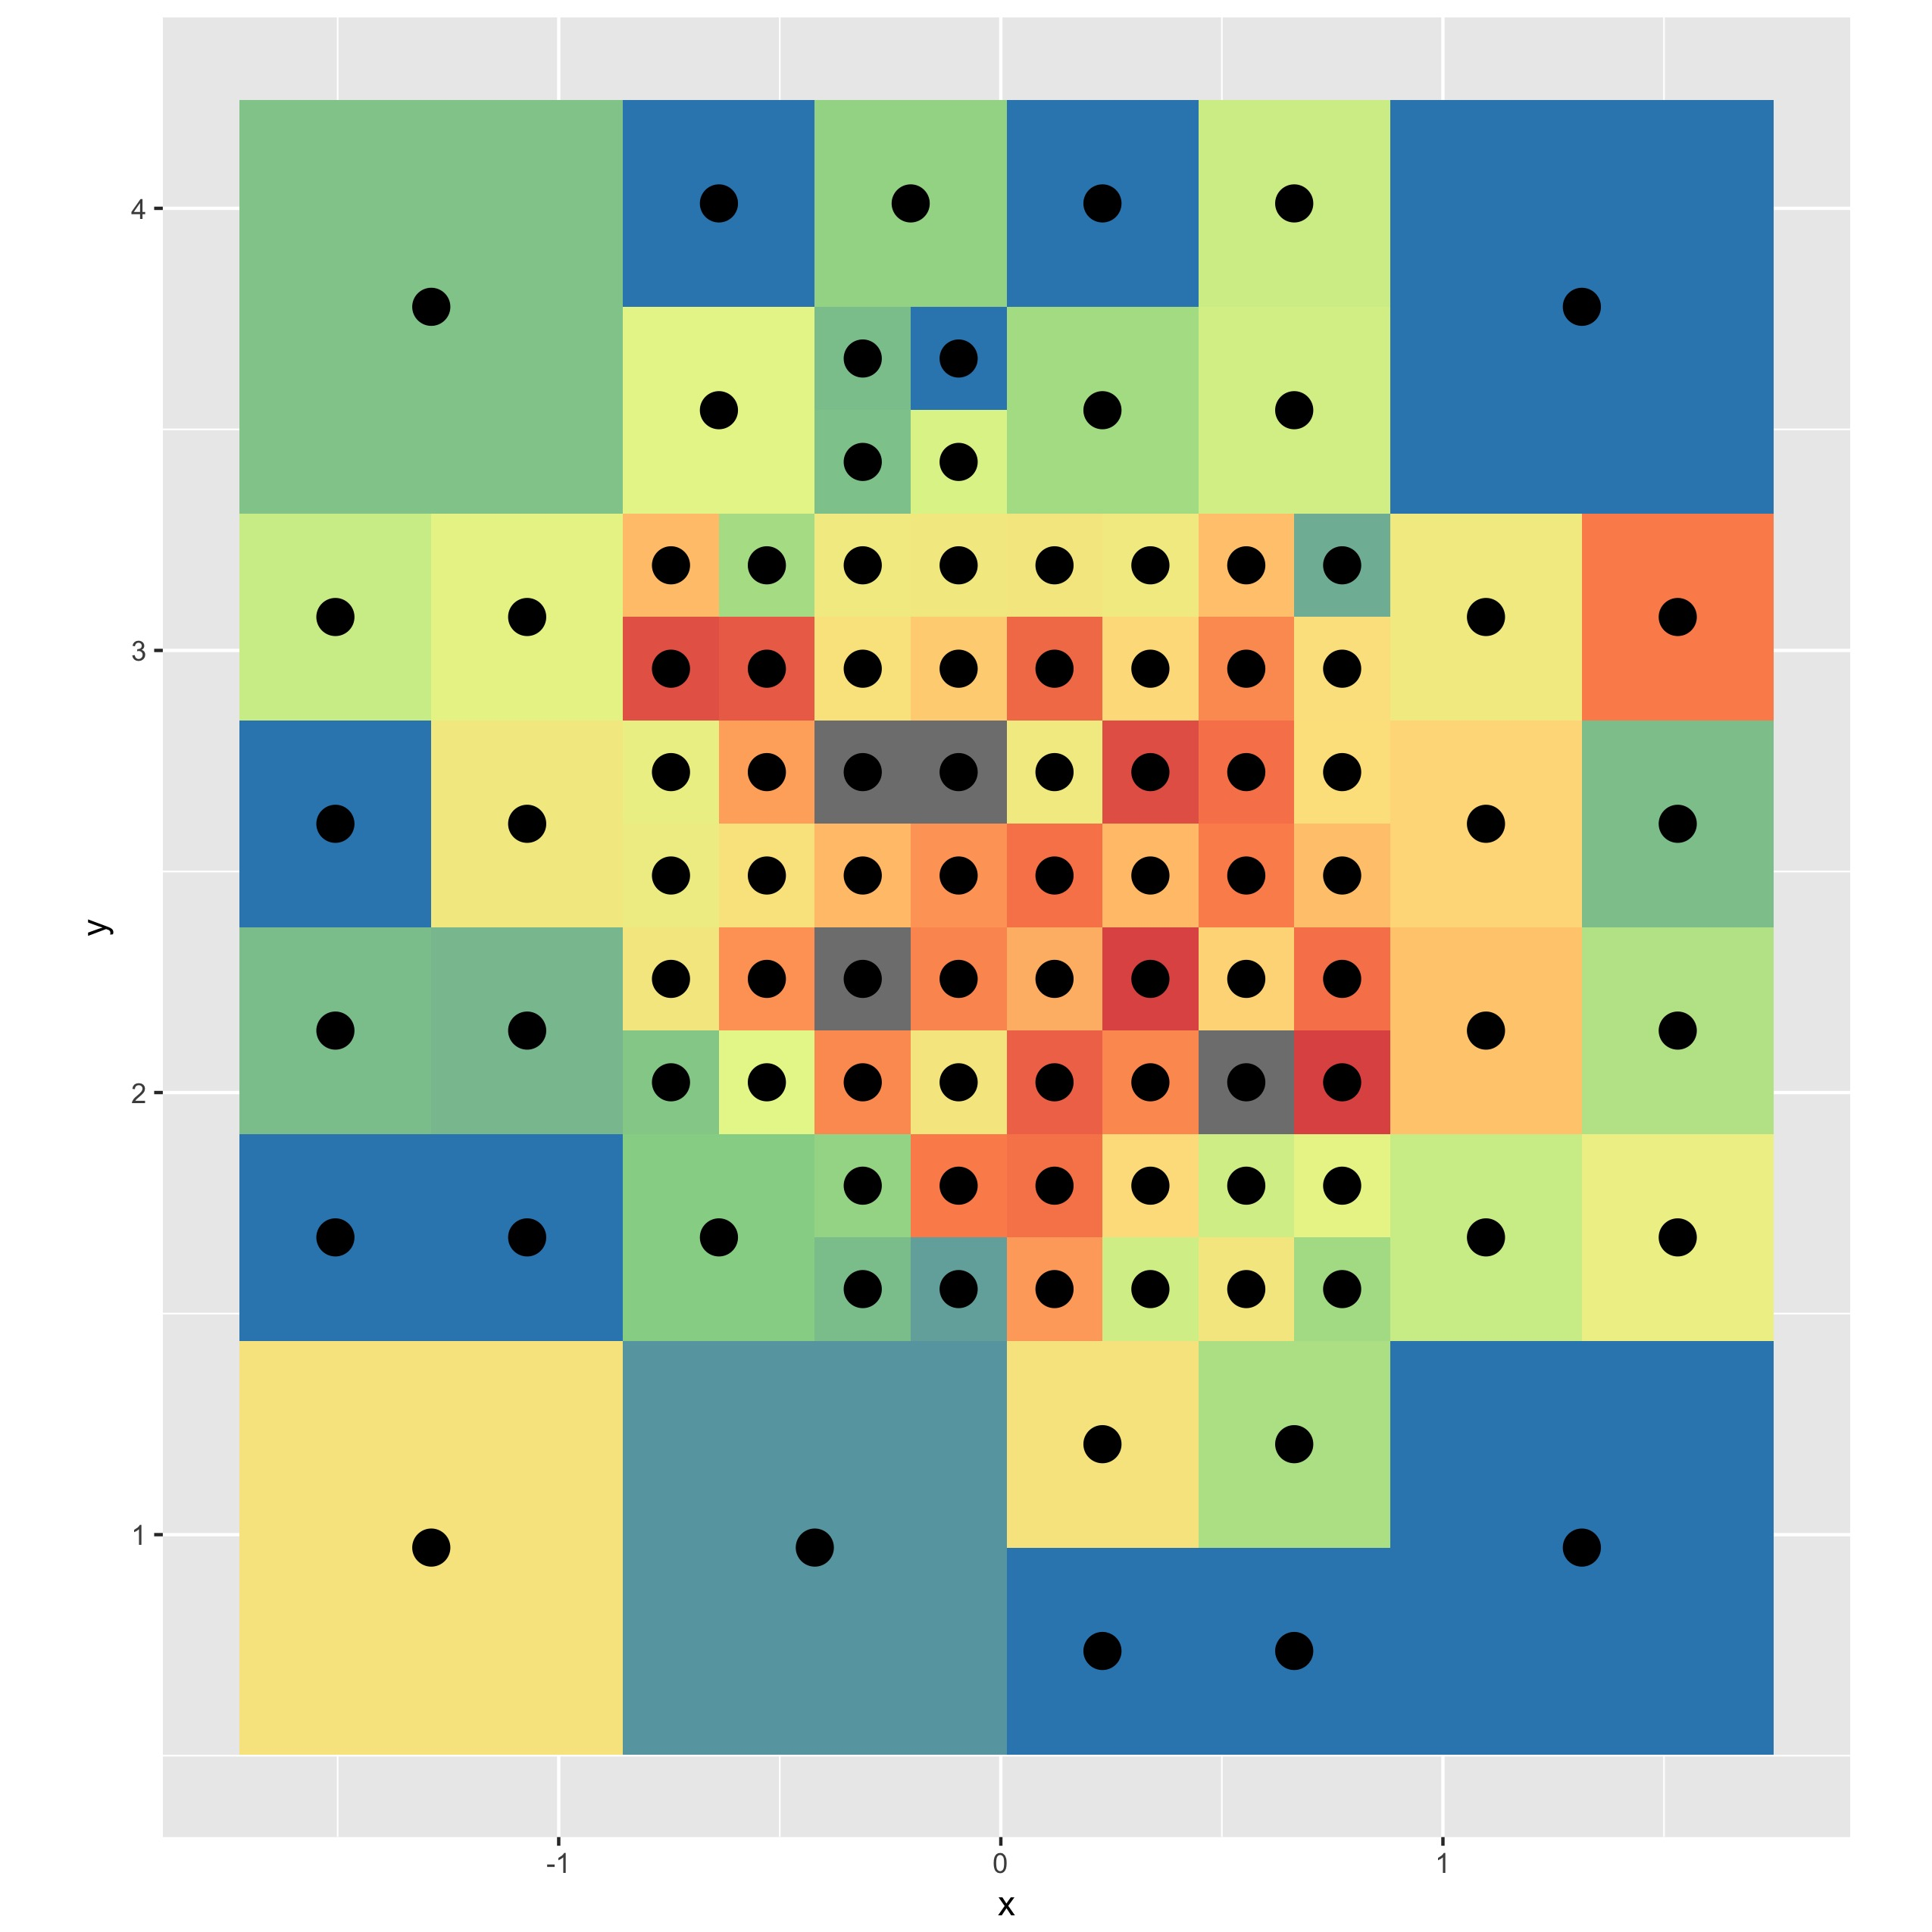
\includegraphics[scale=.08]{Images/knots.jpg}
	\caption{This map shows 97 PPM knots as variable-resolution heat map box centers. This Jhonny Peralta map used stopping rule $n_{b} < 200$.}
	\label{fig:knots}
	\end{figure}
For all results below, we again used a 2012 Macbook Pro with a 2.5 GHz Intel processor, two cores, and 4 GB of RAM. Using the 97 knots in Figure \ref{fig:knots}, for $n = 300$ observations, the \verb|spGLM| function generated 10,000 (nonconvergent) MCMC iterations in three minutes. For $n = 500$ observation, 10,000 (nonconvergent) iterations required 4 minutes. For the same number of knots, but $n = 1000$ observations, 10,000 (nonconvergent) iterations required approximately seven minutes; and 37,500 (nonconvergent) iterations required 23 minutes. 

In our second set of model fits, we chose as knots all 49 VR heat map box centers from the penultimate ($4^{th}$) iteration. Still using $n = 1000$ observations, the \verb|spGLM| function generated 30,000 iterations in seven minutes. For $n = 3000$ observations (still with 49 knots), \verb|spGLM| generated 37,500 iterations in 27 minutes. Notice that the elapsed time increased by only four minutes, despite going from $n = 1000$ to $n = 3000$ observations. This small increase resulted from reducing the number of knots from 97 to 49. These two factors---the number of observations and the number of knots---interactively influence the computational costs. 

These computing times demonstrate the tremendous increase in computational cost over the GLM model fit; and the increase in MCMC iterative speed over model fitting in Stan, where we were unable to fit a model to an n = 3000 observation data set. 

\subsection{Discussion} % ========= ========= =========
These results show promise in terms of MCMC sampling speed, but no MCMC chains converged at our sampling lengths. Recall that the Peralta data set contains 9,172 observations, however, and the final PPM attempt described used only $n = 3000$ of these. Increasing the number of observations beyond 3000 slowed MCMC iterations substantially. Closer to 9000 observations, R sessions stalled and sometimes aborted. Ultimately, we would like a SGLMM fit to all 9,172 observations for comparison to the GLM fit, in order to answer whether a spatial random effect enhances the model sufficiently to justify its inclusion.  

Our goal is a practical model, efficient enough to quickly re-fit with new data in real-time on a personal computer. Ideally, such a model includes more covariates and categories; recall the numerous aspects of the hitter vs. pitcher contest we omitted. With these goals in mind, next we explore an approximation technique that should reduce computation time even further.

% ======== ========= ========= ========= ========= =========
\section{Integrated Nested Laplace Approximations} \label{INLA} 

\subsection{Introduction} % ========= ========= =========

Integrated Nested Laplace Approximation (INLA) works well for parameter estimation in Bayesian hierarchical models with latent Gaussian {\it Markov} random fields (GMRFs), but not directly with GRFs \citep{Rue2007}.

Adding a particular neighborhood structure to a GRF yields a GMRF \citep{Rue2007}. The neighborhood structure explicitly defines when two spatial random effects are neighbors, and the Markov structure assigns non-zero correlation to them if and only if they are neighbors. The importance of the distinction between GRFs and GMRFs lies in the GMRF's sparse precision matrix, because INLA's speedy computations rely on it.

\cite{Lindgren2011} used stochastic calculus \citep{Mao2007} to provide an explicit link between continuous GRFs and discrete GMRFs, and thus made INLA accessible to models with a GRF like ours. Specifically, the stochastic partial derivative of a Mat\'ern GRF equals a Gaussian random field white noise process \citep{Lindgren2011}. This stochastic partial differential equation (SPDE) buttresses a method to approximate a {\it Mat\'ern} GRF with a GMRF, in the form of a piecewise linear basis representation. The approach, known as Finite Element Method (FEM), projects the SPDE onto a basis representation \citep{Dhatt2012}, consisting of deterministic basis functions, defined by a triangulation of the domain, and GMRF weights. This discrete basis representation has a sparse precision matrix, suitable for INLA. 

\subsubsection{Gaussian Markov Random Fields} % ========= =========

To formally define a GMRF , let $\pmb{w}(\pmb{s}) = \{w(\pmb{s}_{i}):i \in V\}$, where $V = \{1,\dots,n\}$. Now define graph $G = \{ V, E \}$, containing vertices $V$ and edges $E$. Vertices $w(\pmb{s}_{i})$ and $w(\pmb{s}_{k})$ are conditionally independent given all other elements of $\pmb{w}(\pmb{s})$, if and only if $\{\pmb{s}_{i}, \pmb{s}_{k}\} \notin E$. The neighborhood structure defined by this graph yields a GMRF, $\pmb{w}(\pmb{s})$, with respect to $G$, where $\pmb{s}_{i} \sim \pmb{s}_{k}$ denotes that $w(\pmb{s}_{i})$ neighbors $w(\pmb{s}_{k})$. The edges in $E$ correspond exactly to the non-zero elements of the GMRF precision matrix $\Sigma$: $\{\pmb{s}_{i}, \pmb{s}_{k}\} \in E$ if and only if $\Sigma_{ik} \neq 0 \text{ for } i \neq k$. Non-zero elements of $\Sigma_{ik}$ correspond to neighbors.

INLA requires that latent random effect $\pmb{w}(\pmb{s})$ be a GMRF. We follow the method of \cite{Lindgren2011}, who use an SPDE to explicitly link a Mat\'ern GRF to a GMRF. 

% ========= ========= ========= ========= ========= 
\subsection{Stochastic Partial Differential Equation (SPDE)} \label{SPDE}

\cite{Whittle1954} declared the $\text{Mat\'ern}_{\nu = 1}$ spatial correlation structure---not the exponential ($\text{Mat\'ern}_{\nu = 1/2}$)---the ``elementary correlation'' function in two dimensions. The following defines the Mat\'ern family of covariance functions.
$$\text{C}\left(w(\pmb{s}_{i}), w(\pmb{s}_{k}) \right)= \frac{\sigma^{2}}{2^{\nu - 1}\Gamma(\nu)}(\kappa ||\pmb{s}_{i} - \pmb{s}_{k}||)^{\nu}K_{\nu}(\kappa ||\pmb{s}_{i} - \pmb{s}_{k}||)$$
This parameterization includes range parameter $\kappa > 0$, smoothness parameter $\nu > 0$, scale parameter $\sigma^{2}$, and modified Bessel function $K_{\nu}(\cdot)$ \citep{Schabenberger2004}.

In order to use INLA, based on \cite{Whittle1954}, \cite{Mondal2017}, and \cite{Lindgren2015}, we now assume a $\text{Mat\'ern}_{\nu = 1}$ covariance structure for the GRF (Equation \ref{eq:w}). This gives the model:
$$ Y_{i}|\mathbf{X}_{i}(\mathbf{s}_{i}) \stackrel{ind}{\sim} \mbox{Bernoulli}(\pi_{i}), $$
$$ \text{logit}(\pi_{i}|\pmb{s}_{i}) = \mathbf{X}_{i}(\mathbf{s}_{i})\beta + w(\pmb{s}_{i}), $$
$$ \pmb{w}(\pmb{s}) | \sigma, \kappa \sim MVN(\pmb{0}, \Sigma(\sigma, \kappa)), $$
for
\begin{equation}
\Sigma_{i,k} = \sigma^{2}(\kappa ||\pmb{s}_{i} - \pmb{s}_{k}||)K_{1}(\kappa ||\pmb{s}_{i} - \pmb{s}_{k}||).
\end{equation}
We adopt a Mat\'ern covariance structure for the GRF because  Mat\'ern random fields solve the SPDE used to explicitly link a GRF to a GMRF \citep{Whittle1954}. The SPDE,
\begin{equation} \label{eq:spde1}
(\kappa^{2} - \Delta)^{\alpha/2}\pmb{w}(\pmb{s}) = \pmb{W}(\pmb{s}),
\end{equation}
includes the Laplace operator $\Delta = \sum_{s_{i}=x_{i},y_{i}} \frac{\partial^{2}}{\partial s_{i}^{2}}$; spatial scale (range) parameter $\kappa$; smoothness parameter $\alpha$; and Gaussian spatial white noise process $\pmb{W}(\pmb{s})$. 

Based on the SPDE-Mat\'ern relationship and $\nu = 1$, we have the following forms for $\alpha$, $\sigma$, and the SPDE:
\begin{align}
\alpha &= \nu + d/2 \nonumber \\
&= 1 +2/2 \nonumber \\
&= 2 \nonumber
\end{align}
where d = 2 because our domain is a subset of $\mathbb{R}^{2}$;
\begin{align}
\sigma^{2} &= \frac{\Gamma(\nu)}{\Gamma(\alpha)(4\pi)^{d/2}\kappa^{2\nu}} \nonumber \nonumber \\
&= \frac{1}{4 \pi \kappa} \nonumber
\end{align}
and 
\begin{equation} \label{eq:spde}
(\kappa^{2} - \Delta)\pmb{w}(\pmb{s}) = \pmb{W}(\pmb{s}).
\end{equation}

To reiterate, until now we assumed an exponential covariance structure for $\pmb{w}(\pmb{s})$. Based on \cite{Whittle1954}; \cite{Mondal2017} and \cite{Lindgren2015}; now we assume a $\text{Mat\'ern}_{\nu = 1}$ covariance structure for the random effect $\pmb{w}(\pmb{s})$. 

% ========= ========= ========= ========= =========
\subsubsection{Piecewise Linear Basis Representation}
The Finite Element Method projects the SPDE onto a piecewise linear basis representation of $\pmb{w}(\pmb{s})$, which we will denote with $\widetilde{\pmb{w}}(\pmb{s})$ \citep{Simpson2012}. The basis representation,
\begin{equation} \label{eq:basisrep}
\widetilde{\pmb{w}}(\pmb{s}) = \sum_{k=1}^{n_{v}} \psi_{k}(\pmb{s})\omega_{k},
\end{equation}
contains deterministic basis functions, $\psi_{k}(\cdot)$; and GMRF weights $\pmb{\omega} = \{\omega_{1},\dots,\omega_{n_{v}}\}$, where $n_{v}$ is the total number of {\it vertices}; let $V_{k}$ represent triangulation vertex $k$ (as described in the next Section, \ref{dbf}). The two combine in \ref{eq:basisrep} so that the distribution of $\widetilde{\pmb{w}}(\pmb{s})$ approximates the Mat\'ern GRF that solves the SPDE, but retains a sparse precision matrix and its accordant computational advantages \citep{Lindgren2011}. 

\subsubsection{Deterministic Basis Function} \label{dbf} % ========= =========

A triangulation of the spatial domain defines the deterministic component, $\psi_{k}(\pmb{s})$, of the basis representation in equation \ref{eq:basisrep}. Figure \ref{fig:basis} shows how a discrete piecewise linear basis function uses domain triangulation to approximate a continuous function \citep{Simpson2012}.
  \begin{figure}[H]
	\centering
	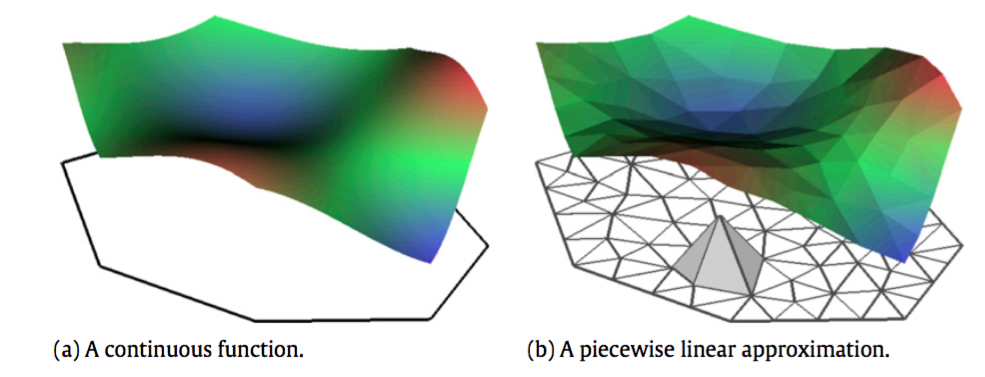
\includegraphics[scale=.4]{Images/PLBF.jpg}
	\caption{A Gaussian Markov random field, defined as the piecewise linear basis function $\pmb{w}(\pmb{s}) = \sum_{k=1}^{n_{v}} \protect\psi_{k}(\pmb{s})\protect\omega_{k}$, approximates a Mat\'ern GRF. This image illustrates how a triangular mesh over the domain determines basis functions $\protect\psi_{k}(\pmb{s})$ (Reproduced from \cite{Simpson2012}).}
	\label{fig:basis}
	\end{figure}
Figure \ref{fig:basis} (b) shows a domain triangulation, under the surface it is used to approximate. In equation \ref{eq:basisrep}, $n_{v}$ represents the number of {\it vertices} in the domain triangulation. The basis functions $\psi_{k}$ are piecewise linear in each triangle, with basis function $k$ equal to one at vertex $k$: $\psi_{k}(V_{k}) = 1$; and basis function $k$ equal to zero at all other vertices: $\psi_{k}(V_{k'}) = 0$ for $k'\neq k$. This implies that the approximation at vertex $k$, $\widetilde{\pmb{w}}(V_{k})$,  is equal to the value of the GRF weight, $\omega_{k}$, at that vertex.
\begin{align}
\widetilde{\pmb{w}}(V_{k}) &= \psi_{k}(V_{k}) \omega_{k} \\
&= 1 \cdot \omega_{k}
\end{align}
For points $\pmb{s}$ located in triangle interiors, $\widetilde{\pmb{w}}(\pmb{s})$ equals a linear combination of the GRF weights, $\omega$, at the three vertices that form the containing triangle. That is, for triangle $T$ made from vertices $t_{1}, t_{2}, t_{3}$; location $\pmb{s} \in T$; and constants $c_{1}, c_{2}, c_{3}$:
\begin{align}
\widetilde{\pmb{w}}(\pmb{s}) &= \psi_{t_{1}}(\pmb{s})\omega_{t_{1}} + \psi_{t_{2}}(\pmb{s})\omega_{t_{2}} 
+ \psi_{t_{2}}(\pmb{s})\omega_{t_{2}} \nonumber \\
&= c_{1}\omega_{t_{1}} + c_{2}\omega_{t_{2}} 
+ c_{3}\omega_{t_{2}} \nonumber
\end{align}

\subsubsection{Gaussian Weights} % ========= ========= =========

Stochastic calculus identities provide a way to calculate the weights, $\omega$, in the basis representation of \ref{eq:basisrep}. To start, define notation: $$\langle f(\pmb{u}, g\pmb{u}) \rangle = \int f(\pmb{u}) g(\pmb{u}) d\pmb{u}.$$ 
Then find weights $\pmb{\omega}$ such that, for a set of test functions $\phi_{k}$ where $k = 1, \dots, n_{*}$, the following distributional equality of integral random vectors holds \citep{Lindgren2011}:
\begin{equation}  \label{eq:stoch} % =======
\left[ \left< \phi_{l}, (\kappa^{2} - \Delta) \pmb{w} \right> \right]_{l = 1, \hdots, n_{*}} 
\overset{D}{=}
\left[ \langle \phi_{l}, \pmb{W} \rangle \right]_{l = 1, \hdots, n_{*}}.
\end{equation}

The solution---weight vector $\pmb{\omega}$ in basis representation $\widetilde{\pmb{w}}$ (equation \ref{eq:basisrep})---gives the stochastic weak solution solution to the SPDE in Equation \ref{eq:spde} \citep{Mao2007}, \citep{Lindstrom2014}. 

We follow \cite{Lindgren2011} and use the {\it Galerkin} solution, where the deterministic basis functions, $\psi_{k}$,  of section \ref{dbf} serve as test functions: $\phi_{k} = \psi_{k}$. Substituting these into \ref{eq:stoch} gives:

\begin{equation} \label{eq:stoch2} % =======
\left[ \left< \psi_{l}, (\kappa^{2} - \Delta) \pmb{w} \right> \right]_{l = 1, \hdots, n_{v}} 
\overset{D}{=}
\left[ \langle \psi_{l}, \pmb{W} \rangle \right]_{l = 1, \hdots, n_{v}}.
\end{equation}

Then, substitute the basis function representation in Equation \ref{eq:basisrep}, $\widetilde{\pmb{w}}$, in for $\pmb{w}$ and simplify:
% $\widetilde{w} = \Sigma_{k}\psi_{k}w_{k}$:

% \left[ \left< \psi_{l}, (\kappa^{2} - \Delta) \left( \sum_{k=1}^{n_{v}} \psi_{k}\omega_{k} \right) \right> \right]_{l = 1, \hdots, n_{*}} \overset{D}{=} \Big[ \langle \psi_{l}, \pmb{W} \rangle \Big]_{l = 1, \hdots, n_{*}}.

$$ \left[ \left< \psi_{l}, (\kappa^{2} - \Delta) \left( \sum_{k=1}^{n_{v}} \psi_{k}\omega_{k} \right) \right> \right]_{l = 1, \hdots, n_{v}} 
\overset{D}{=}
\left[ \langle \psi_{l}, \pmb{W} \rangle \right]_{l = 1, \hdots, n_{v}} $$

$$ \left[ \left< \psi_{l}, (\kappa^{2} - \Delta) \psi_{k} \right> \right]_{l,k} \pmb{\omega} 
\overset{D}{=} 
\Big[ \langle \psi_{l}, \pmb{W} \rangle \Big]_{l} $$ 

$$  \left[ \left< \psi_{l}, (\kappa^{2}\psi_{k} - \Delta \psi_{k})  \right> \right]_{l,k} \pmb{\omega} 
\overset{D}{=} 
\Big[ \langle \psi_{l}, \pmb{W} \rangle \Big]_{l}  $$

$$ \Big( \kappa^{2} [ \langle \psi_{l}, \psi_{k} \rangle ] + [ \langle \psi_{l}, -\Delta \psi_{k} \rangle ] \Big) \pmb{\omega} 
\overset{D}{=} 
\Big[ \langle \psi_{l}, \pmb{W} \rangle \Big]_{l} $$

Simplify notation by letting $\pmb{C} = \langle \psi_{l}, \psi_{k} \rangle$, and $ \pmb{G} = \langle \psi_{l}, - \Delta \psi_{k} \rangle$, to give

$$ \left(
\kappa^{2} \pmb{C} + \pmb{G} \right) \pmb{\omega} \overset{D}{=} \Big[ \langle \psi_{l}, \pmb{W} \rangle \Big]_{l}.$$

The {\it Galerkin} solution\footnote{For additional details and proofs see \cite{Lindgren2011}: pages 429 - 431, Appendix A and Appendix C.} gives $\Big[ \langle \psi_{l}, \pmb{W} \rangle \Big]_{l} \sim \text{N}(\pmb{0},\pmb{C})$, so that
$$ \left(
\kappa^{2} \pmb{C} + \pmb{G} \right) \pmb{\omega} \overset{D}{=} \text{N}(\pmb{0},\pmb{C}).$$

Thus, $\pmb{\omega} \sim \text{N}(\pmb{0}, \pmb{Q}^{-1})$ for precision matrix
\begin{equation} \label{eq:Q}
\pmb{Q} = \left( \kappa^{2} \pmb{C} + \pmb{G} \right)^{T} \pmb{C}^{-1} \left( \kappa^{2} \pmb{C} + \pmb{G} \right).
\end{equation}

$\pmb{C}^{-1}$ has a sparse precision matrix, however the same is not necessarily true of $\pmb{C}$. Therefore, replace $\pmb{C}$ in equation \ref{eq:Q} with diagonal matrix $\widetilde{\pmb{C}}$:
$$ \widetilde{\pmb{C}}_{i,i} = \langle \psi_{i}, \pmb{1} \rangle = \int \psi_{i}(\pmb{s}) d\pmb{s}.$$
\begin{equation} \label{eq:Q2}
\pmb{Q} = \left( \kappa^{2} \widetilde{\pmb{C}} + \pmb{G} \right)^{T} \pmb{C}^{-1} \left( \kappa^{2} \widetilde{\pmb{C}} + \pmb{G} \right).
\end{equation}

Note that this solution specifies the distribution of the vector of weights $\pmb{\omega}_{k}$ in the piecewise linear basis function representation of $\widetilde{\pmb{w}}(\pmb{s})$ (equation \ref{eq:basisrep}), not the distribution of $\widetilde{\pmb{w}}(\pmb{s})$ itself.

% ========= ========= ========= ========= ========= =========
\subsection{Integrated Nested Laplace Approximations (INLA)}

To explain INLA in this section, define hyperparameter vector $\pmb{\theta} = \{\kappa, \sigma \}$; parameter vector $\pmb{\rho} = \{ \pmb{\beta}^{\text{T}}, \widetilde{w} \}^{\text{T}}$; and let $\pmb{Q}$ denote the precision matrix of $\pmb{\rho}$.

INLA estimates the marginal posterior distributions for latent field parameters, $p(\rho_{i}|\pmb{y})$; and covariance hyperparameter posterior $p(\pmb{\theta}|\pmb{y})$. This means INLA does not estimate posteriors $p(\pmb{\rho}|\pmb{y})$ and $p(\pmb{\rho},\pmb{\theta}|\pmb{y})$. We break the INLA procedure into three steps to facilitate explanation.

\subsubsection{Step 1, Gaussian Approximation} % ======= ======

INLA begins by ``matching the mode and curvature at the mode'' of Gaussian estimator $p_{G}(\pmb{\rho}|\pmb{\theta}, \pmb{y})$ to that of $p(\pmb{\rho}|\pmb{\theta}, \pmb{y})$ \citep{Rue2005}. Note that INLA requires Gaussian priors for all parameters in $\pmb{\rho}$, excluding covariance hyperparameters in $\pmb{\theta}$. INLA also requires conditional independence: $p(\pmb{y}|\pmb{\rho}, \pmb{\theta}) = \prod_{i} p(y_{i}|\pmb{\rho}_{i},\pmb{\theta})$. In our case, with a spatial random effect, if we condition on the random effect, we essentially fix it, and thus what remains is independent. Therefore 
\begin{align}
p(\pmb{\rho} |\pmb{\theta},\pmb{y}) & \propto p(\pmb{y}|\pmb{\rho}, \pmb{\theta}) p(\pmb{\rho}|\pmb{\theta}) p(\pmb{\theta}) \nonumber \\
p(\pmb{\rho}|\pmb{\theta},\pmb{y}) & \propto \text{exp}\left(-\frac{1}{2}\pmb{\rho}^{T}\pmb{Q \rho} + \sum_{i} \text{log }p(y_{i}|\pmb{\rho}_{i},\pmb{\theta}) \right). \nonumber
\end{align}
Assuming Gaussian priors and conditional independence, the INLA Gaussian approximation for $p(\pmb{\rho}|\pmb{\theta}, \pmb{y})$ takes the form
\begin{equation} \label{eq:ga}
p_{G}(\pmb{\rho}|\pmb{\theta},\pmb{y}) \propto \text{exp} \left( -\frac{1}{2}(\pmb{\rho-\mu})^{T} (\pmb{Q} + \text{diag}(\pmb{c}) ) (\pmb{\rho - \mu}) \right),
\end{equation}
where the vectors $\pmb{c}$ and $\pmb{\mu}$ depend on second order Taylor expansions of $f(\pmb{\rho}) = \sum_{i} \text{log }p(y_{i}|\pmb{\rho}_{i},\pmb{\theta})$ about the mode \citep{Lindstrom2014}. A Newton-Raphson algorithm iteratively computes the mode and precision matrix until convergence \citep{Rue2009}. Step 2 uses the approximation in \ref{eq:ga} to approximate $p(\pmb{\theta}|\pmb{y})$.

\subsubsection{Step 2, Laplace Approximation}  % ====== ======

This step begins with two sides of a familiar identity, and its subsequent rearrangement. Recall conditional probability rules give the two equalities for $p(\pmb{y} , \pmb{\rho} | \pmb{\theta})$:
\begin{enumerate}
\item $p(\pmb{y} , \pmb{\rho} | \pmb{\theta}) = p(\pmb{\rho} | \pmb{y}, \pmb{\theta}) p(\pmb{y} | \pmb{\theta})$. 
\item $p(\pmb{y} , \pmb{\rho} | \pmb{\theta}) = p(\pmb{y} | \pmb{\rho}, \pmb{\theta}) p(\pmb{\rho} | \pmb{\theta})$
\end{enumerate} 
Linking these together we have
$$ p(\pmb{y} , \pmb{\rho} | \pmb{\theta}) = p(\pmb{\rho} | \pmb{y}, \pmb{\theta}) p(\pmb{y} | \pmb{\theta}) = p(\pmb{y} | \pmb{\rho}, \pmb{\theta}) p(\pmb{\rho} | \pmb{\theta}),$$
and removing ``$p(\pmb{y} , \pmb{\rho} | \pmb{\theta})$'' from the far left-hand side leaves
$$ p(\pmb{\rho} | \pmb{y}, \pmb{\theta}) p(\pmb{y} | \pmb{\theta}) = p(\pmb{y} | \pmb{\rho}, \pmb{\theta}) p(\pmb{\rho} | \pmb{\theta}). $$
Now divide both sides by ``$p(\pmb{\rho} | \pmb{y}, \pmb{\theta})$'' to get 
\begin{equation}
p(\pmb{y} | \pmb{\theta}) = \frac{p(\pmb{y} | \pmb{\rho}, \pmb{\theta}) p(\pmb{\rho} | \pmb{\theta})} {p(\pmb{\rho} | \pmb{y}, \pmb{\theta})}.
\end{equation}
Next, substitute this last formulation of $p(\pmb{y}|\pmb{\theta})$ into Bayesian theorem:
\begin{align}
p(\theta|\pmb{y}) & \propto p(\pmb{y}|\pmb{\theta})p(\pmb{\theta}) \nonumber \\
& \propto \frac{p(\pmb{y} | \pmb{\rho}, \pmb{\theta}) p(\pmb{\rho} | \pmb{\theta})}{p(\pmb{\rho} | \pmb{y}, \pmb{\theta})} \cdot p(\pmb{\theta})
\end{align}
For a given $\pmb{\theta}$, let $\pmb{\rho}_{0} = \text{argmax}_{\rho}p(\pmb{\rho}|\pmb{y},\pmb{\theta})$. Then,
\begin{equation} \label{eq:la}
p(\pmb{\theta}|\pmb{y}) \approx \tilde{p}(\pmb{\theta}|\pmb{y}) \propto  \frac{p(\pmb{y} | \pmb{\rho}_{0}, \pmb{\theta}) p(\pmb{\rho}_{0} | \pmb{\theta})}{p_{G}(\pmb{\rho}_{0} | \pmb{y}, \pmb{\theta})} \cdot p(\pmb{\theta}),
\end{equation}
with the Taylor approximation of $f(\pmb{\rho}) = \sum_{i} \text{log }p(y_{i}|\rho_{i})$ in $p_{G}(\pmb{\rho} | \pmb{y}, \pmb{\theta})$ expanded about $\pmb{\rho}_{0}$. Then, we have approximate maximum likelihood estimate $\hat{\pmb{\theta}}_{\text{ML}} \approx \text{argmax}_{\theta} \tilde{p}(\pmb{\theta}|\pmb{y})$. \cite{Tierney1986} showed this approximation matches the Laplace approximation. 
Next, in Step 3, we use the results of Step 1 and Step 2 to nest and numerically integrate the Laplace approximations to obtain approximate marginal posteriors.

\subsubsection{Step 3, Numerical Integration} % === === === === ===
Using the Gaussian approximation, $p_{\text{G}}(\rho_{j}|\pmb{\theta, y})$, from equation \ref{eq:ga} in Step 1; and the Laplace approximation, $\tilde{p}(\pmb{\theta}|\pmb{y})$, from equation \ref{eq:la} in Step 2; we can now integrate numerically to find posterior marginals $p(\rho_{i}|\pmb{y})$ and $p(\theta_{i}|\pmb{y})$. 
        $$ p(\rho_{j} | \pmb{y}) \approx \int p_{\text{G}}(\rho_{j}|\pmb{\theta, y})\tilde{p}(\pmb{\theta}|\pmb{y}) d\pmb{\theta} $$
        $$ p(\theta_{k} | \pmb{y}) \approx \int \tilde{p}(\pmb{\theta}|\pmb{y}) d\pmb{\theta}_{-k} $$
        
For additional details of the procedure, see \cite{Rue2009}. We implement the SPDE-INLA procedure of the previous two subsections with the function \verb|inla()| in the R package {\bf INLA} \citep{INLA}, \citep{Lindgren2015}.
        
\subsection{Results}
The INLA model fit with n = 1000 observations required approximately 5 seconds; and the n = 3000 fit required approximately 9 seconds. Most impressively, the INLA fit to all 9177 Peralta observations required approximately 34 seconds. In Figure \ref{fig:INLA} we show the VR heat map, GLM fit heat map, and the INLA fit heat map.
  \begin{figure}[H]
	\centering 	
	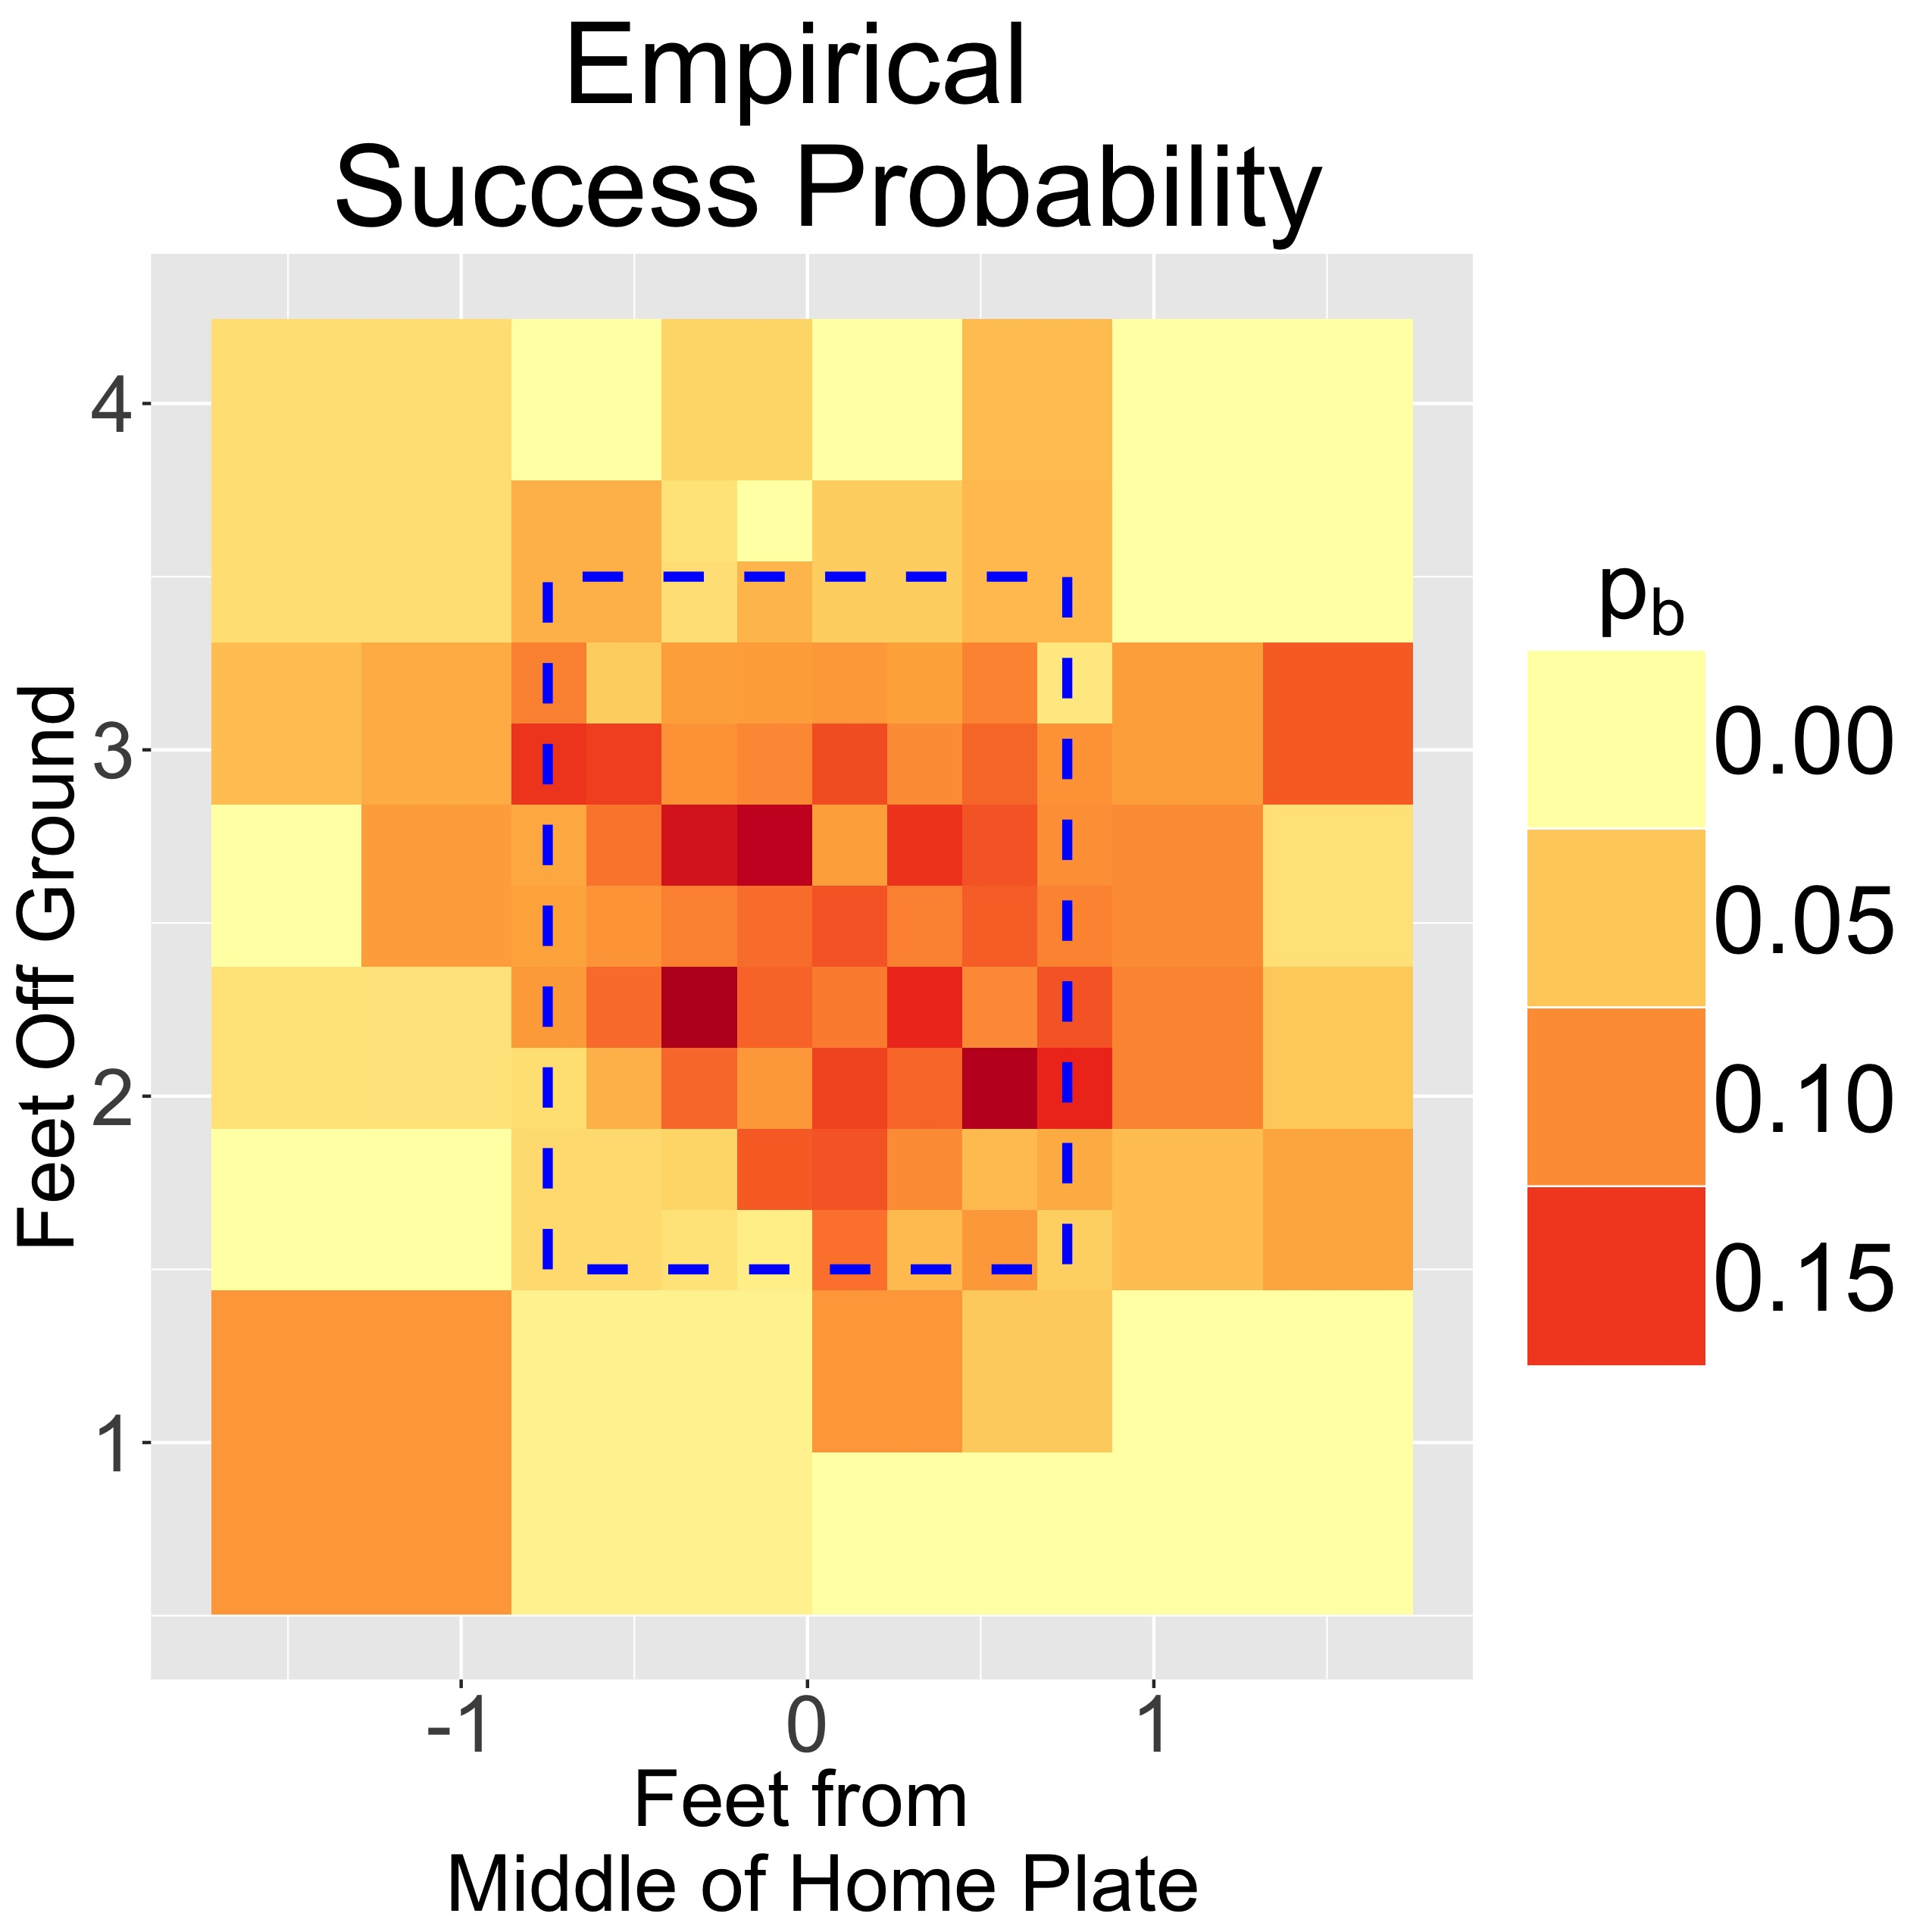
\includegraphics[scale=.05]{Images/Peralta_var-res2.jpg}
	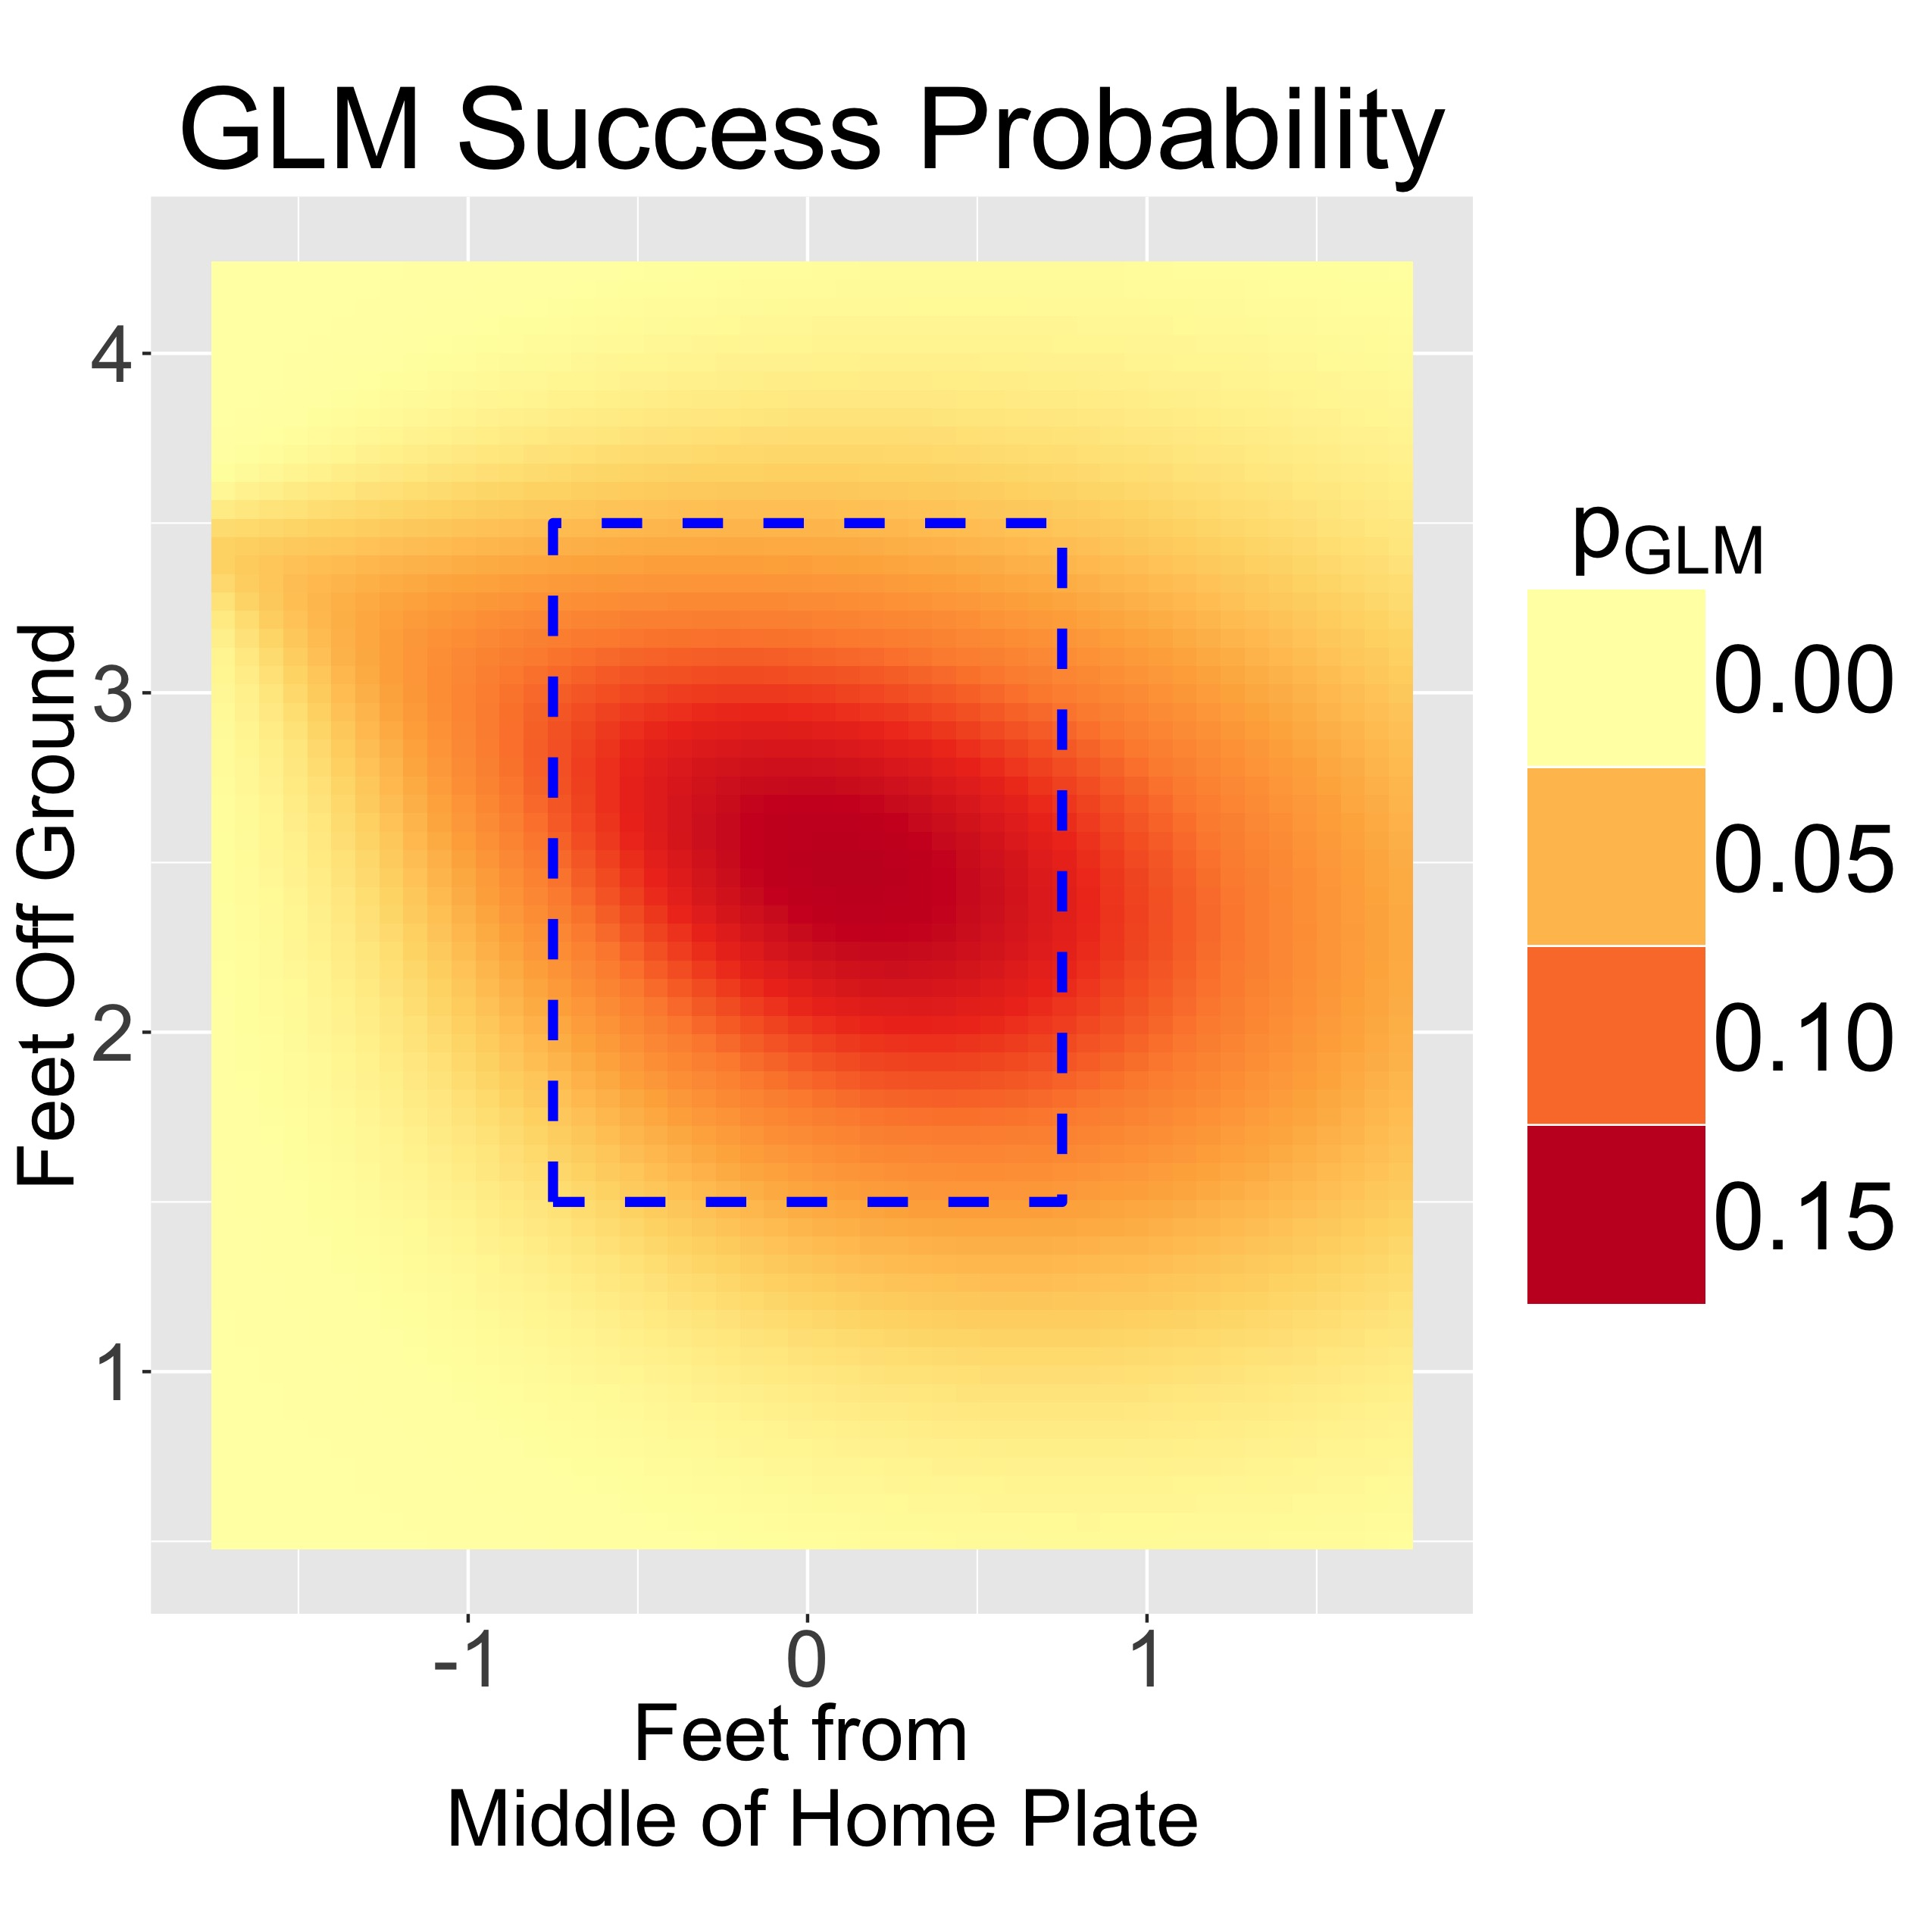
\includegraphics[scale=.05]{Images/Peralta_fit.jpg}
	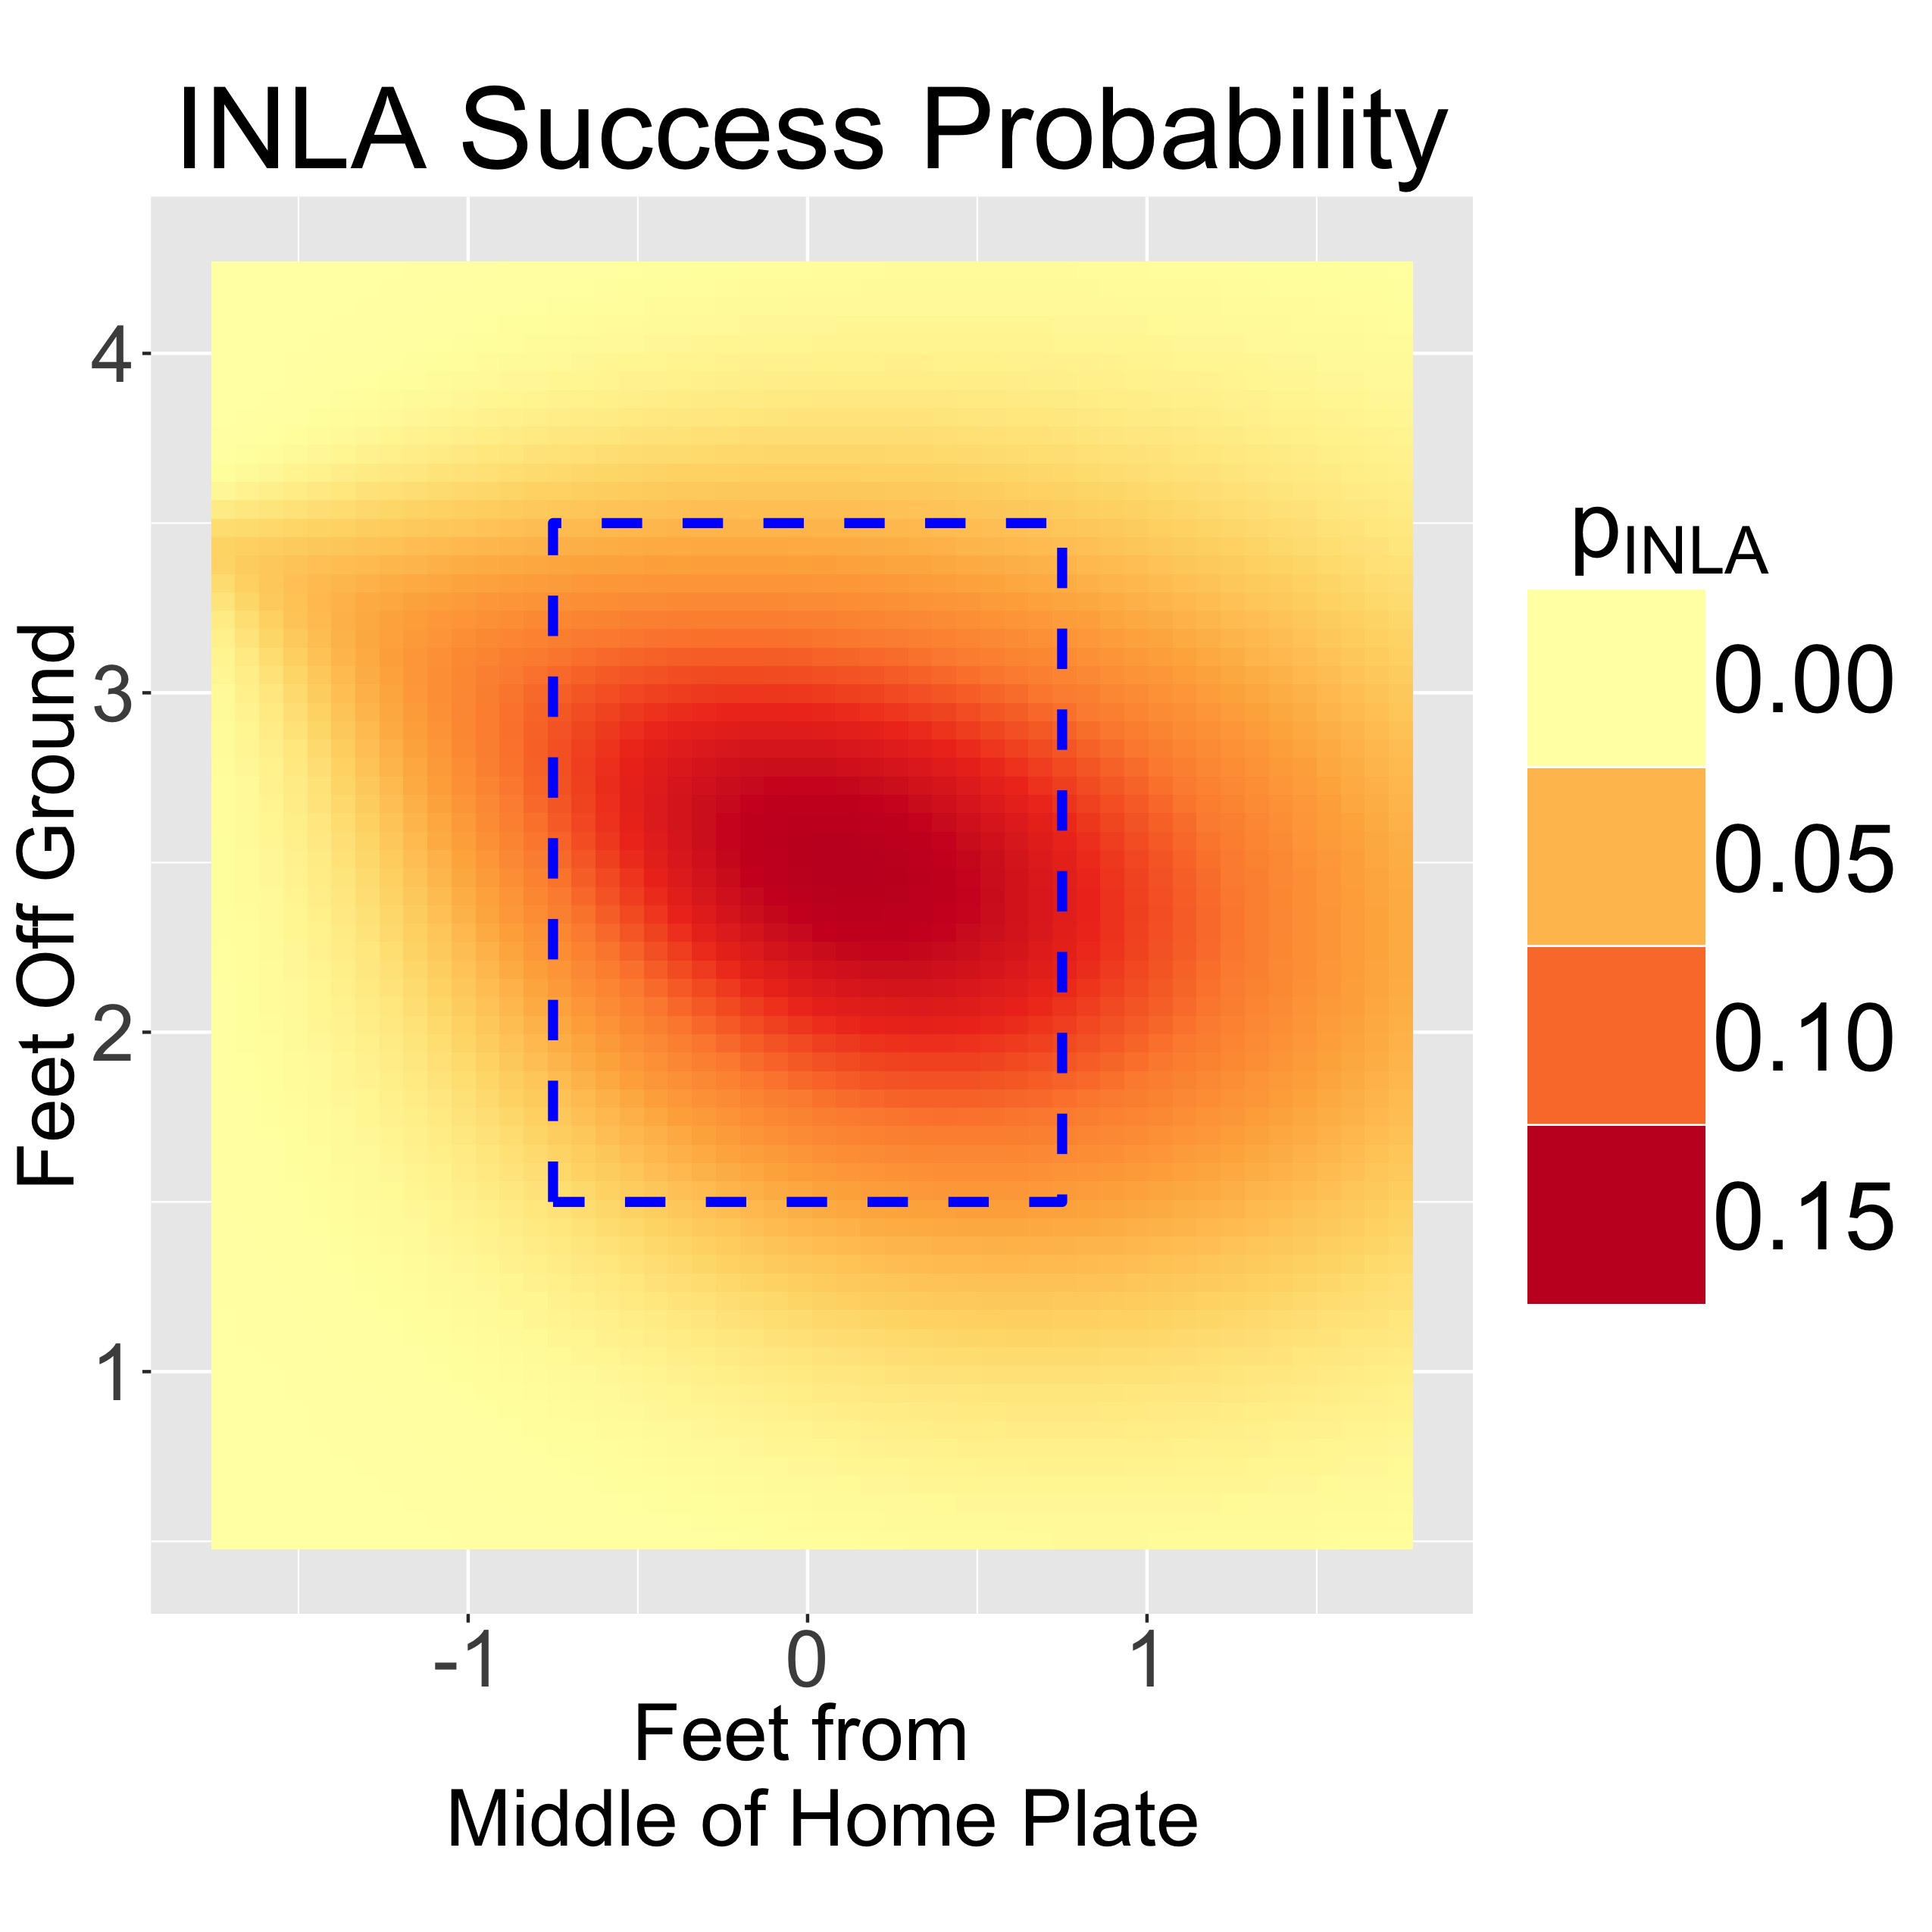
\includegraphics[scale=.05]{Images/INLA.jpg}
	\caption{VR heat map, GLM fit heat map, and Integrated Nested Laplace Approximation (INLA) model fit heat map. The INLA fit with all n = 9177 Peralta observations required approximately 34 seconds.}
	\label{fig:INLA}
	\end{figure}
The fit resembles the empirical map with approximately the same degree of similarity as the GLM. The GLM and INLA fit heat maps are very similar. We show GLM and INLA estimates in the tables below for comparison.  \\

\begin{tabular}{| l | c | c | c |}
\hline
\multicolumn{4}{|c|}{} \\
\multicolumn{4}{|c|}{} \\
\multicolumn{4}{|c|}{GLM} \\
\hline
Covariate         & $\beta_{i}$ & MLE   & SE   \\ \hline
1                 & $\beta_{0}$ & -4.08 & 0.70 \\ \hline
r                 & $\beta_{1}$ &  1.19 & 0.51 \\ \hline
$\theta$          & $\beta_{2}$ & -1.93 & 1.90 \\ \hline
$r*\theta$        & $\beta_{3}$ & -1.64 & 0.70 \\ \hline
$r^{2}$           & $\beta_{4}$ & -0.32 & 0.09 \\ \hline
$\theta^{2}$      & $\beta_{5}$ & -3.92 & 1.10 \\ \hline
$r^{2}*\theta^{2}$& $\beta_{6}$ & -0.46 & 0.21 \\ \hline
\end{tabular}
\quad
\begin{tabular}{| l | c | c | c |}
\hline
\multicolumn{4}{|c|}{INLA} \\
\hline
Covariate         & $\rho _{i}$ & $\hat{\rho}_{i}$ & SE \\ \hline
N/A               & $\kappa$    &  3.23 & $\pm$ 1 SE: (1.35, 7.54) \\ \hline
N/A               & $\sigma$    &  0.11 & $\pm$ 1 SE: (0.05, 0.26) \\ \hline
1                 & $\beta_{0}$ & -4.14 & 0.76 \\ \hline
r                 & $\beta_{1}$ &  1.25 & 0.55 \\ \hline
$\theta$          & $\beta_{2}$ & -1.90 & 1.96 \\ \hline
$r*\theta$        & $\beta_{3}$ & -1.70 & 0.93 \\ \hline
$r^{2}$           & $\beta_{4}$ & -0.33 & 0.10 \\ \hline
$\theta^{2}$      & $\beta_{5}$ & -3.93 & 1.14 \\ \hline
$r^{2}*\theta^{2}$& $\beta_{6}$ & -0.48 & 0.22 \\ \hline 
\end{tabular} \\

The coefficient estimates and SEs are very similar for the GLM and INLA model fits. The INLA Mat\'ern covariance parameter estimate $\hat{\kappa}$ indicates long range correlation, albeit at a low scale indicated by $\hat{\sigma} = 0.11$.

Most noteworthy, the INLA fit succeeded for this larger data set. The model fits required quantities of time sufficiently small to allow amateur and professional experimentation on personal computers, achieving one of our goals.

\section{Conclusion}
In this chapter we saw that optimized Stan code and PPMs both inadequately address the computational burden of fitting an SGLMM to our data. Our final approach, INLA, approximates parameters and thereby avoids the $\mathcal{O}(n^{3})$ computational burden of using MCMC to fit SGLMMs. INLA fit the SGLMM to all n = 9177 observations, in 34 seconds.

PPMs necessarily sacrifice some spatial information in reducing dimensionality. This dimension reduction possibly contributed to non-convergence; trace plots indicated non-convergence of most parameters after 30,000 draws with n = 97 knots and n = 1000 observations. Despite requiring 60 minutes for as many observations, Stan fit trace plots exhibited no such convergence difficulties. In future attempts to use PPMs, convergence diagnostics should precede substantive modeling and analysis for inference. The \verb|CODA| package offers diagnostic tools to assess mixing, autocorrelation, and convergence, such as the Gelman-Rubin convergence diagnostic \citep{CODA}, \citep{Gelman2014}, \citep{Brooks1998}

Partially counterbalancing its model fitting speed, INLA for spatial Bernoulli data yields biased estimators \citep{Mondal2017}. Therefore, using INLA for further research and inference will require, like PPM, preliminary steps. These steps should include simulation analysis of the bias characteristics, and a literature review of the topic including the discussion in \cite{Rue2007}. In addition, a thorough examination of estimate variance characteristics should follow. Creating an interactive HMCI in {\bf mapapp} would help compare the variance of INLA estimates to the variance of GLM estimates.

When satisfactory model fitting occurs, model comparison of GLMs and SGLMMs fit with INLA should follow. Comparisons can follow the example of \cite{Finley2009_2}, and use probability model scoring rules to compare fits \citep{Bickel2007}, \citep{Gneiting2007}. The essential question to answer: does the random effect enhance the model sufficiently to justify the increased computational costs?

In summary, this chapter reviewed and detailed three approaches to fitting SGLMMs to big N, spatial, strike zone data. Future researchers, depending on goals and speed requirements, can bypass model fitting in Stan; focus on convergence and convergence diagnostics of long MCMC runs for PPM fitting; and investigate INLA variance properties as just described. 
